\chapter{Computational Implementation} \label{chap:implementation}

	The principles of thermodynamic equilibrium set the background for solving phase equilibrium problem in multicomponent system but being able to solve the resulting optimisation problem requires the use of high-quality software implementations. Though several such softwares exists, most of them do not meet the requirements for direct integration with MOOSE framework. The commercial softwares do not provide source codes and the application programming interfaces (APIs) provided by a few of such codes are usually very difficult to modify to meet the needs of multiphysics implementations. The open-source softwares on the other hand do have readily available source codes but often lack in terms of quality of code implementation and software quality assurance (SQA). To overcome the challenges and to provide readily usable thermodynamic equilibrium framework in MOOSE, a new Gibbs energy minimiser was developed.  While many of the algorithms employed in {\GEM} embody the concepts previously presented in open literature, there remains a scope for improving the efficiency and capabilities of some of these algorithms through careful implementation and/or building upon them. The top level architecture of the thermodynamic equilibrium solver has been outlined in figure~\ref{fig:structure}. The program essentially consists of parsing and input modules to read the required thermodynamic data and system information followed by initialisation routines which provide the initial assemblage to a non-linear solver. The assemblage from the non-linear solver is then checked to ensure global minimum is achieved at which stage the outputs are produced.
	\begin{figure}[htbp]
	 	\centering
	   	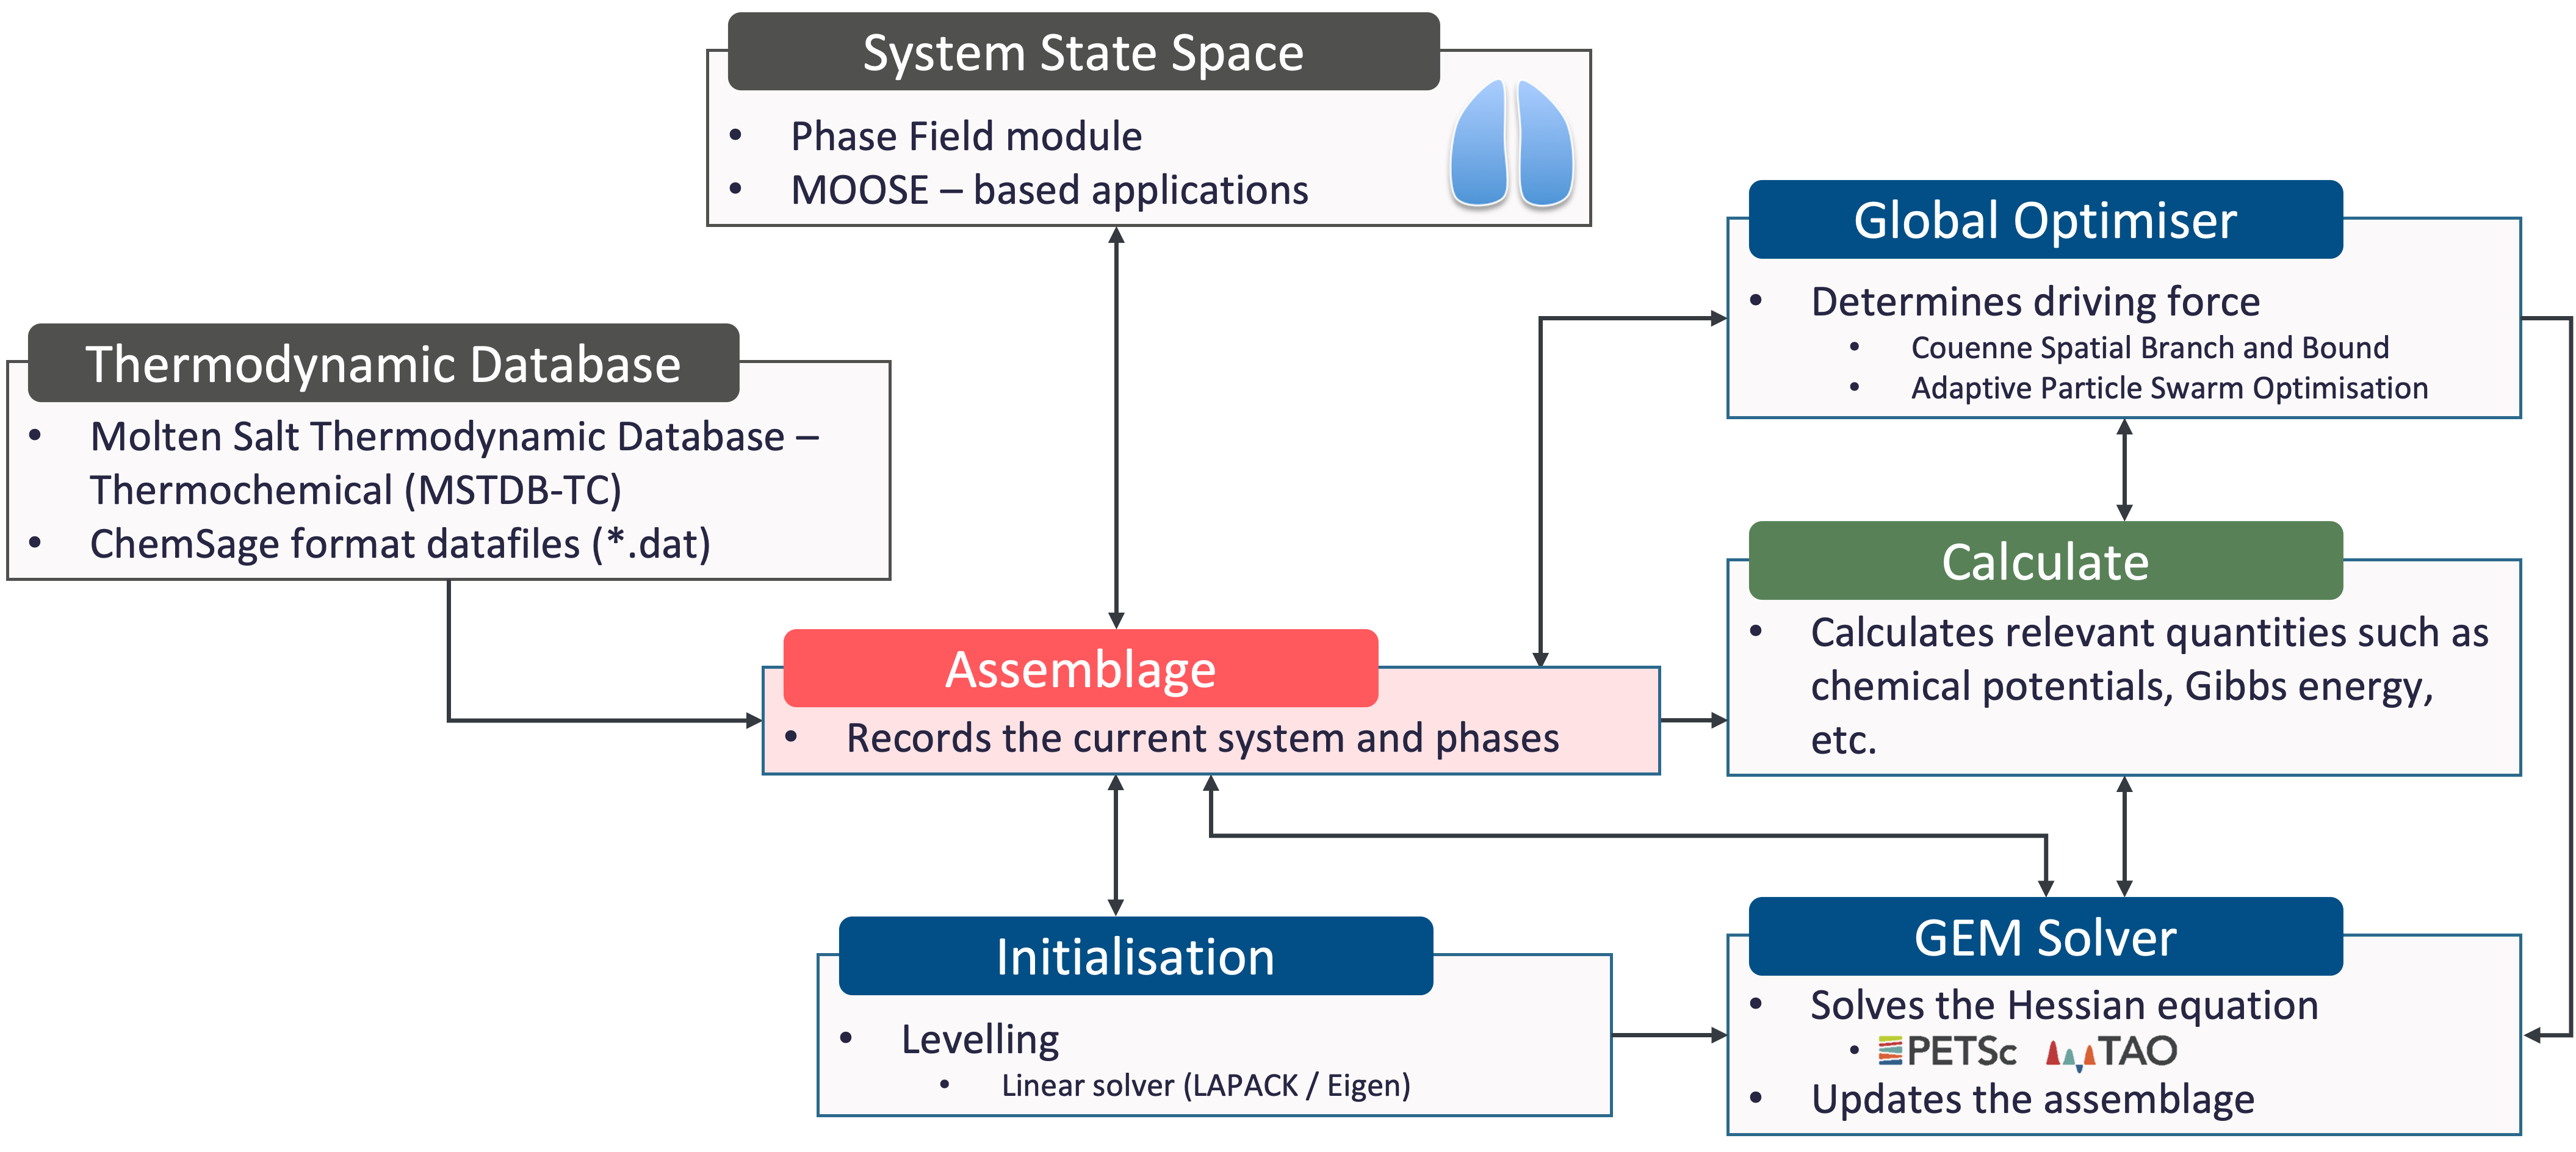
\includegraphics[width=0.95\textwidth]{figures/chapter-6/YJ_structure.png}
	   	\caption{Top-level architecture of \GEM.}
	   	\label{fig:structure}
	\end{figure}


\section{Thermodynamic Database}
	Calculation of thermodynamic equilibrium requires a thermodynamic database, which includes Gibbs energy functions of the different phases and species that can exist in the system. These thermodynamic databases are developed using the well established CALPHAD method \cite{liu_wang_2016} and are available in different formats, the most commonly used being ThermoCalc (*.tdb) and ChemSage (*.dat) data file formats, which are generated by the commercial software ThermoCalc and FactSage, respectively. An example of a typical ChemSage data file is shown in figure~\ref{fig:datfile} and consists of a header block followed by information blocks for every possible phase in the system.
	\begin{figure}[htbp]
	 	\centering
	   	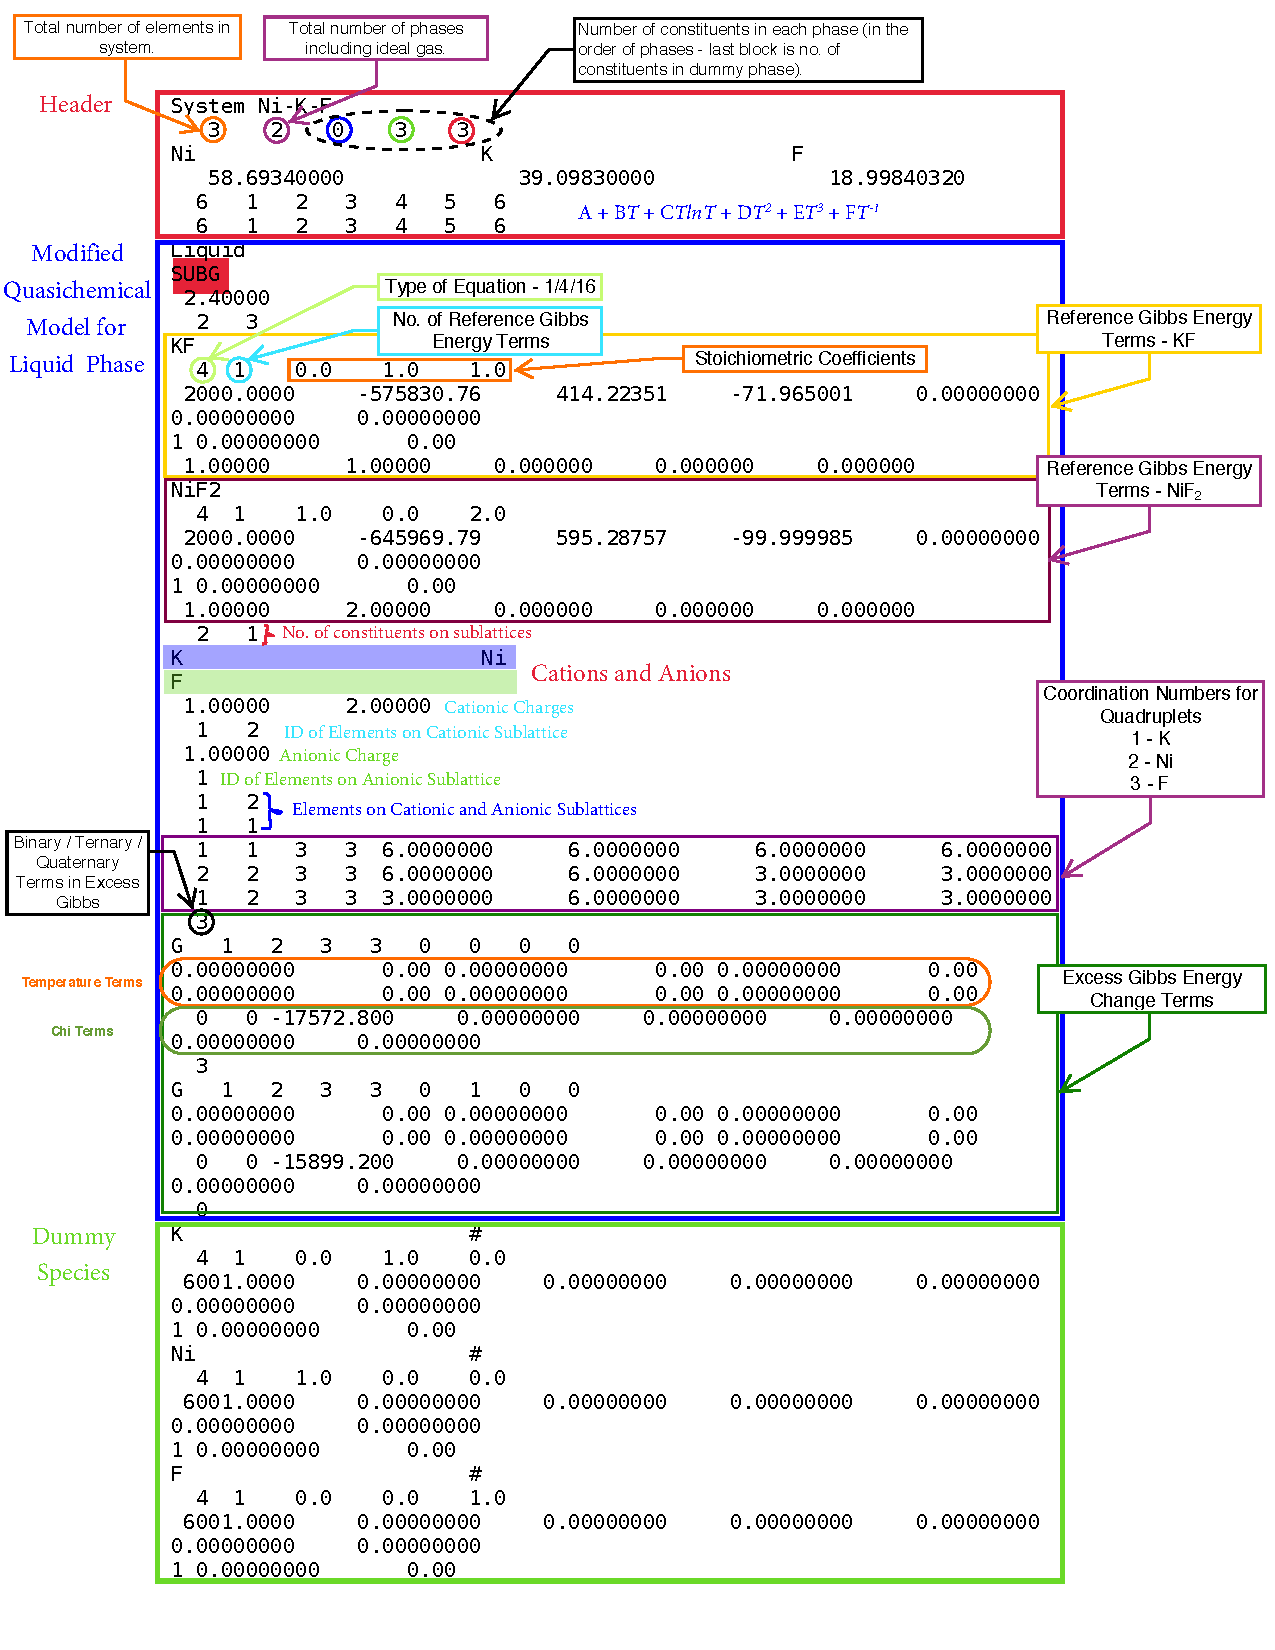
\includegraphics[width=\textwidth]{figures/NiKF.pdf}
	   	\caption[A marked-up example of a ChemSage data file of the \ce{Ni-K-F} system.]{A marked-up example of a ChemSage data file of the \ce{Ni-K-F} system \cite{OcadizFlores18}}
	   	\label{fig:datfile}
	\end{figure}

	A data file parser for {\GEM} has been developed in C++ and it performs the extraction of Gibbs energy functions from ChemSage format (*.dat) thermodynamic files (ChemSage format) and creates an in-memory thermodynamic database class, \texttt{Database}, that can be conveniently accessed by any part of the code throughout rest of the solve. All the data structure objects inherit from a single base class allowing the rest of the code to track the phases conveniently without having to track the model-specific  details. Moreover, in multiphysics simulations, it allows a single database instance to be created at the start of the simulations instead of the need of reading the datafile every time the information is needed. In {\GEM}, the Molten Salt Thermodynamic Database - Thermochemical \cite{MSTDB}, is natively supported but any ChemSage format datafile can be supplied by the user.
	
	The \texttt{Database} class includes a number of utility functions for post-processing and cleaning up the raw database constructed after parsing. A peculiarity of ChemSage datafiles is how they denote phases that can have a miscibility gap. In ChemSage, such phases are denoted by adding a duplicate entry for a phase that is considered to have miscibility gaps. This has several disadvantage. First, this creates unnecessary duplication of thermodynamic data and can have memory and performance implications for large databases. Second, the decision for miscibility gap should be enforced using physical rules rather than basing them upon the database or user inputs. As an example, since a phase with more than one miscibility gap not only plausible but also observed in many physical systems, a phase being duplicated once doesn't reveal any information about the number of such possible gaps and can be a source of confusion. In post-processing, such duplicate entries are deleted, but to not lose the information completely, a flag is raised in the thermodynamic phase whose duplicate was deleted. For multi-sublattice phases, the post-processor also maps all the sublattice constituents to the system components, and, for phase represented by MQM, it calculates the default coordination numbers for the quadruplets that are not included in the datafile.
	
\section{System State-Space}
	Thermochemical equilibrium calculations are isothermal, isobaric point calculations and require the temperature, pressure as well as the composition if the system to be specified. In {\GEM}, this information is provided by MOOSE or MOOSE-based applications such as the Phase Field module. To facilitate such data transfer, a MOOSE UserObject, namely \texttt{GEMUserObject}, has been developed. The MOOSE UserObject system is built for developing and running custom algorithms that may not fit well within any other system in MOOSE. Examples include complex calculations that may result values that don't associate in a one to one manner with elements, nodes, or sides. \texttt{GEMUserObject} allows the thermodynamic equilibrium solver to be called by other codes and the invocation requires that the temperature, pressure and composition be specified as required parameters. The UserObject is also responsible for passing back the return values to the calling code and some of the common variables that are often requested include the Gibbs energy, chemical potentials, stable phases and their speciation.

\section{Initialisation}
	Much like any other optimisation problem, the choice of initial estimate plays a critical role in reducing the amount of computational time required for the solution to converge to a minimum. This requirement of initial estimates of the stable  phases and their speciation creates a significant challenge. Many early softwares created for the purpose of estimating thermodynamic equilibrium, for example SOLGASMIX, required the user to input an initial estimate but this relied on the user's intuition and was often very inconvenient for them, especially when working with complex systems and/or systems where finding estimates from intuition was not straightforward. A bigger problem was that it could often result in initial estimates which were far from the real stable assemblage of phases and would increase the computational cost substantially, often even compromising the convergence itself. 

	To overcome the need for user prescribed initial estimates, Eriksson and Thompson \cite{Eriksson89} proposed an initialisation algorithm called \emph{levelling} that has found widespread application in thermodynamic equilibrium softwares. {\GEM} implements this algorithm as the standard initialisation routine and the it is described in the following text.
	
	\subsection{Levelling}
	The levelling algorithm was developed to accelerate the rate of convergence by eliminating the phases and species that have an insignificant contribution in the final phase assemblage. The algorithm is based on a temporary treatment of all species and phases in the system as pure stoichiometric phases. Mathematically, this amounts to temporarily converting the non-linear optimisation problem into a linear optimisation problem and the algorithm for the computational implementation has been illustrated in figure~\ref{fig:levelling}.
	\begin{figure}[ht]
		\centering
		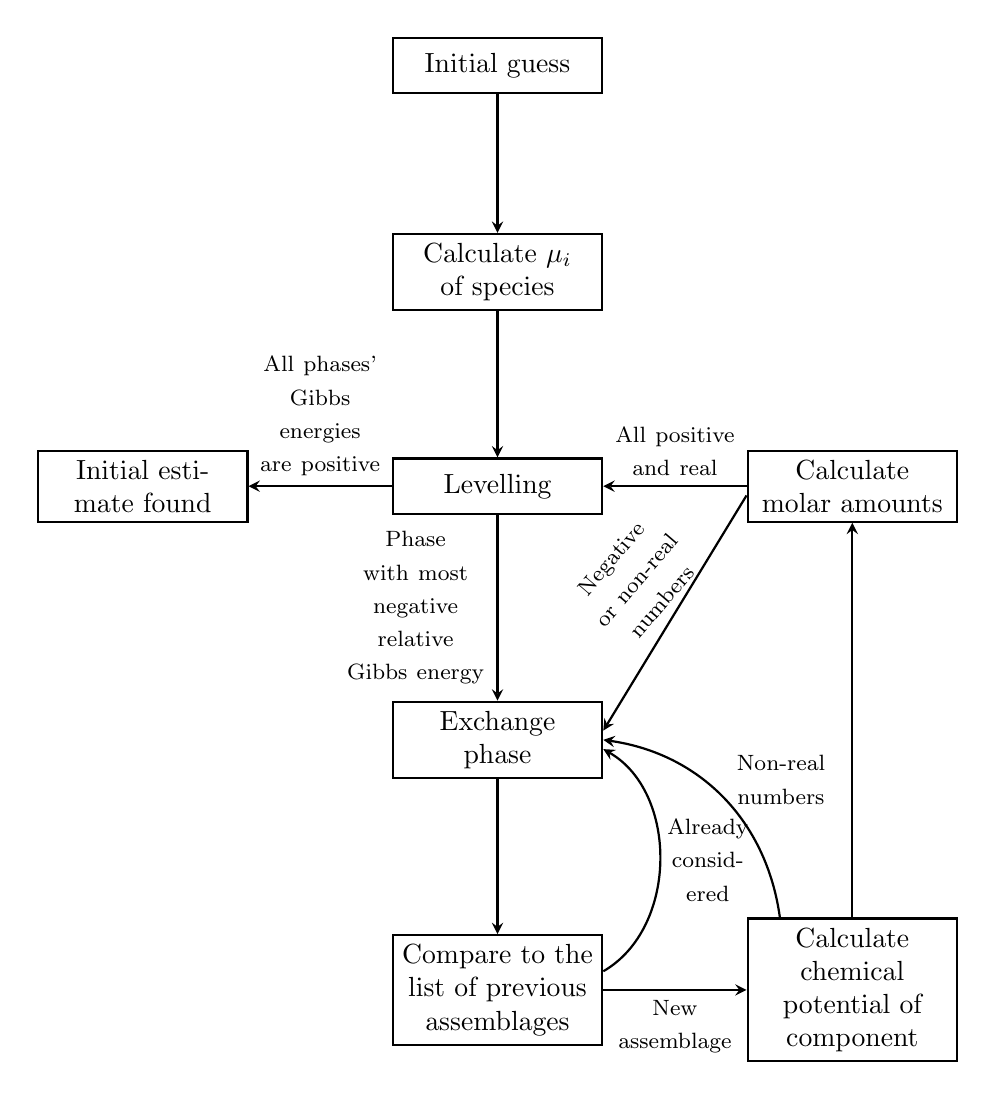
\begin{tikzpicture}[auto,
    			block_center/.style ={rectangle, draw=black, thick, fill=white, text width=0.2\textwidth, text centered, minimum height=2em},
    			block_side/.style ={rectangle, draw=black, thick, fill=white, text width=0.2\textwidth, text centered, minimum height=2em},
			block_noborder/.style ={rectangle, draw=none, thick, fill=none, text width=0.15\textwidth, text centered, minimum height=0.5em},
			block_small/.style ={rectangle, draw=none, thick, fill=none, text width=0.1\textwidth, text centered, minimum height=0.5em},
			line/.style ={draw, thick, -stealth}]
    			% Outlining the flowchart using the PGF/TikZ matrix funtion
    			\matrix [column sep=0.15\textwidth,row sep=5em] {
      				{} & \node [block_center] (01) {Initial guess}; & {}\\
      				{} & \node [block_center] (11) {Calculate $\mu_i$ of species}; & {}\\
      				\node [block_side] (20) {Initial estimate found}; & \node [block_center] (21) {Levelling}; & \node [block_side] (22) {Calculate molar amounts};\\
      				{} & \node [block_center,yshift=-1cm] (31) {Exchange phase}; & {}\\
      				{} & \node [block_center] (41) {Compare to the list of previous assemblages}; & \node [block_side] (42) {Calculate chemical potential of component};\\
    			};	% end matrix
    			% connecting nodes with paths
    			\begin{scope}[every path/.style=line]
      				\path (01) edge (11);
     				\path (11) edge (21);
      				\path (21) edge node[block_noborder,anchor=east]{\footnotesize{Phase with most negative relative Gibbs energy}} (31);
      				\path (31) edge (41);
      				\path (22) edge node[block_noborder,anchor=south]{\footnotesize{All positive and real}} (21);
      				\path (21) edge node[block_noborder,anchor=south]{\footnotesize{All phases' Gibbs energies are positive}} (20);
      				\path (41) edge node[block_noborder,anchor=north]{\footnotesize{New assemblage}} (42);
      				\path (42) edge (22);
      				\path[-] (22.185) edge node[block_noborder,rotate=49.5,anchor=south]{\footnotesize{Negative or non-real numbers}} (31.5);
      				\path[-] (41.10) edge[bend right=60] node[block_small,anchor=west,shift={(-0.125cm,0)}]{\footnotesize{Already considered}} (31.355);
     				\path[-] (42.135) edge[bend right=37] node[block_small,anchor=west,shift={(0,0.225cm)}]{\footnotesize{Non-real numbers}} (31.360);
    			\end{scope}
 		\end{tikzpicture}
  		\caption[Levelling algorithm for finding the initial estimate of stable phase assemblage.]{Levelling algorithm for finding the initial estimate of stable phase assemblage. After Loukusa \cite{Loukusa:2014aa}.}
  		\label{fig:levelling}
 	\end{figure}

	Since the Gibbs energy is a relative thermodynamic function and the Gibbs energies of each component element are not related to one another \cite{Eriksson89}, it is possible to numerically alter the Gibbs energy of each phase while preserving the elemental differences. Levelling is performed by representing the set of Gibbs energies relative to the collection of phases assumed to be most stable and uses a relative Gibbs energy function called the \textit{absolute Gibbs energy} by Eriksson and Thompson and is the Gibbs energy of the pure species per atom in the species as shown in equation~\eqref{eq:absGibbs}
	\begin{equation}\label{eq:absGibbs}
		\hat{G}_i = \frac{G_j}{\sum_{j=1}^C \nu_{ij}}
	\end{equation}

	The levelling process determines the combination of phases yielding the lowest Gibbs energy by evaluating a combination of Gibbs energies on a relative basis. A phase that has a negative relative Gibbs energy with respect to the assemblage indicates that a phase in the assemblage must be replaced by the current phase to achieve a lower integral Gibbs energy.

	Mathematically, levelling is achieved through an iterative process that systematically adjusts fixed combinations of phases, subject to the linear equality and inequality mass balance constraints, to progressively minimise the GIbbs energy of the system \cite{Piro12a}. At iteration $m+1$, the adjustment to be applied to the relative Gibbs energy of phase $i$ is defined by \cite{Eriksson89}:
	\begin{equation} \label{eq:lev_adj}
		\begin{aligned}
			d \hat{G}_i^{m\rightarrow m+1} &= \sum_{j=1}^{C} c_{ij} d \Gamma_j^{m\rightarrow m+1}\\
			\hat{G}_i^{m+1} &= \hat{G}_i^{m} - d \hat{G}_i^{m\rightarrow m+1}
		\end{aligned}
	\end{equation}
	where, $c_{ij}$ denotes the atomic fraction of element $j$ in species $i$ and $d \Gamma_j^{m\rightarrow m+1}$ is the adjustment applied to the chemical potential of element $j$, which in turn is determined by the most stable phases found at iteration $m$.

	In  matrix form, the overall mass balance constraint can be represented as \cite{Piro12a}
	\begin{equation} \label{eq:levMB_mat}
		\mathbf{A^T} \mathbf{n}= \mathbf{b}
	\end{equation}
	where $\mathbf{A} \in \mathbb{R}^{E \times \Phi}$ represents the stoichiometric matrix, $\mathbf{n} \in \mathbb{R}^{\Phi }$ denotes the column vector of the number of moles of each phase, and $\mathbf{b} \in \mathbb{R}^{E}$ is the column vector with the total mass of each element in the system. When equation~\ref{eq:levMB_mat} is used in levelling, $\Phi = E$.

	The initial guess for the levelling method is the most chemically stable form of each element and the stoichiometric matrix $\mathbf{A^T}$ in equation~\eqref{eq:levMB_mat} becomes a diagonal matrix. Subsequently, provided all elements of vector $\mathbf{b}$ are positive, all the elements of $\mathbf{n}$ must also be positive. However, the diagonality of the stoichiometric matrix is not preserved over subsequent iteration and it assumes a non-symmetric sparse form. In fact, the matrix $\mathbf{A^T}$ might become rank deficient if proper care is not taken while selecting the phase assemblage.

	In levelling, since the number of phases in the system is equal to the number of elements, the element potentials can then be uniquely determined from the current estimated phase assemblage by solving the following system of linear equations:
	\begin{equation} \label{eq:levEP_mat}
		\mathbf{A^T} \boldsymbol{\Gamma} = \boldsymbol{\mu}
	\end{equation}
	where $\boldsymbol{\Gamma} \in \mathbb{R}^{E} $ and $\boldsymbol{\mu} \in \mathbb{R}^{\Phi}$.

	The next step in levelling is updating the phase assemblage in accordance with equation~\eqref{eq:lev_adj}. A  species with a positive $\hat{G}_i^{m+1}$ would yield a thermodynamically less stable assemblage and is left out along with phases with insignificant contributions to final equilibrium while the phase with the most negative $\hat{G}_i^{m+1}$ is introduced into the assemblage by replacing a phase in the previous assemblage. The phase assemblage at this stage must meet three requirements. First, the number of moles of all phase in $\mathbf{n}$ must be non-negative and real. Second, all the elements of the vector $\boldsymbol{\Gamma}$ must be real. Finally, the phase assemblage must not have been previously considered. If the phase assemblage does not meet any of these requirements, the phase with the second lowest relative Gibbs energy must be considered, and so on.

	While the criteria for the phase to be added in the system was well established by Eriksson and Thompson, a criterion to select the phase to be replaced wasn't proposed and, typically, local iterations were performed to systematically traverse through the candidate phases until a particular combination yielded an entire set of non-negative and real mole numbers \cite{Eriksson89}. The number of these local iterations rapidly grows with the number of elements in the system and an alternative named \emph{Euclidean norm} was proposed by Piro and Simunovic \cite{Piro12a}. This method has been described in sec.~\ref{sec:Euclidean}

	Once the new phase has been exchanged with one of the existing phases and its acceptability has been determined, levelling step is repeated until no phases with negative absolute Gibbs energy remain in the system. At this stage, the assemblage can be passed on to a non-linear solver as the initial estimate.


	\begin{figure}[htbp]
		\centering
		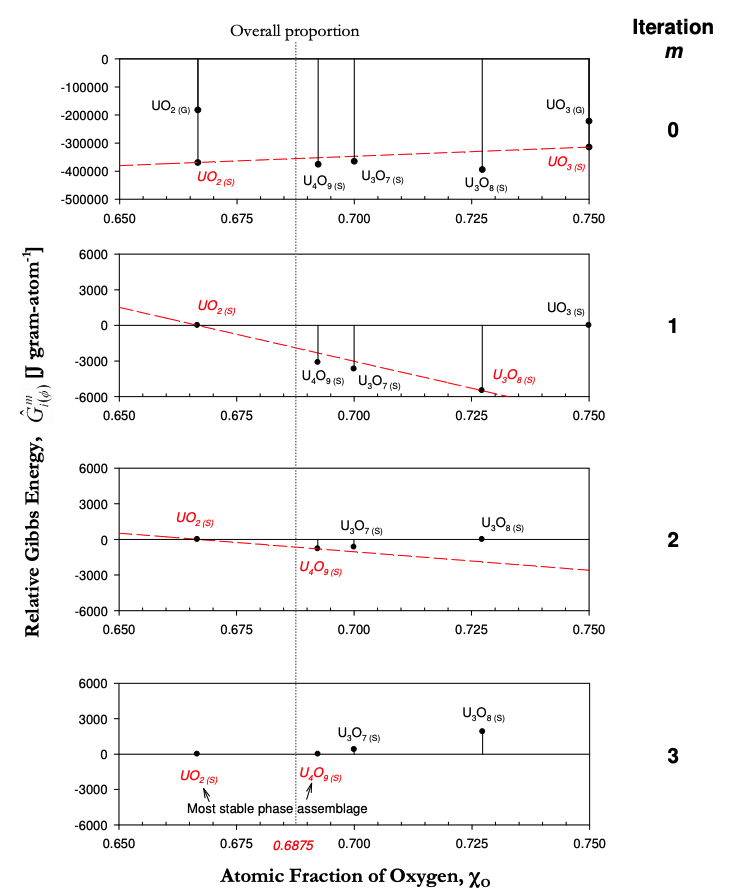
\includegraphics[width=\textwidth]{figures/Levelling_illustration}
		\caption{Illustration of the levelling process for a binary system of \ce{U-O} at each iteration (1 \si{\mole} \ce{U}, 2.2 \si{\mole} \ce{O}, 298.15 \si{\kelvin}, 1 \si{atm}) \cite{Piro11b}.}
		\label{fig:lev_illus}
	\end{figure}

	An example of the levelling method is presented in figure~\ref{fig:lev_illus}. In the illustration, in the first iteration, the phase with the most negative Gibbs energy is paired with another phase that together has non-negative molar quantities. At the end of iteration 0, choosing solid \ce{UO2} as the phase with the most negative relative Gibbs energy and arbitrarily choosing solid \ce{UO3} to pair it with, the equivalent Gibbs energies of pure uranium and pure oxygen are computed and followed by the element potentials $\Gamma_{\ce{U}}$ and $\Gamma_{\ce{O}}$ (represented by the dashed red line). The levelling procedure is then applied and the relative Gibbs energies of the terms are calculated.

	At the start of iteration 1, the relative Gibbs energy of solid \ce{U3O8} is negative with respect to the combination of solid \ce{UO2} and solid \ce{UO3}, indicating it must be introduced in the assemblage. The internal linear solver then determines the phase that must be replaced and the iterative process continues with the updated phase assemblage.

	At the end of the levelling procedure, the assemblage has the lowest Gibbs energy with all other phases being positive with respect to the assemblage. The Gibbs energy of the pure stoichiometric system is thereby minimised. For the example presented in figure~\ref{fig:lev_illus}, the levelling solver converges in only 3 iterations. According to Eriksson and Thompson \cite{Eriksson89}, the computational expense using levelling can be up to two to five times lower than the general equilibrium calculations.

	Mathematically, the levelling  process always respects the Gibbs phase rule, mass balance and the Gibbs' criterion and the number of iterations required to achieve convergence is typically close to the number of elements. This results in significant computational advantage when considering exceeding large number of possible phase combinations as the number of elements in the system grow making levelling an excellent choice as an initialisation routine.

%	\subsection{Post-levelling}
%	Developed by Piro and Simunovic \cite{Piro12a}, the post-levelling method is an extension to the levelling method and can be used to refine the assemblage provided by the levelling method by accounting for the ideal mixing of the phases and relaxing the assumption that the phases are pure. Thus, post-levelling acts as an intermediate step between levelling and the non-linear solver. While post-levelling resembles the non-linear solver in the incorporation of compositional component in the chemical potential of the solution phase constituents, the primary distinction between them is that post-levelling considers only dominant phases identified by levelling as compared to the non-linear solver which considers all the constituents. Furthermore, the non-linear solver also considers non-ideal behaviour.
%
%		The chemical potential term in post-levelling takes the following form:
%		\begin{equation}
%			\begin{aligned}
%				\mu_{i(\lambda} &= g_{i(\lambda)}^0 + RT \ln{(x_{i(\lambda)})} \\
%				x_{i(\lambda)} &= \frac{n_{i(\lambda)}}{\sum_{k=1}^{N_{\lambda}}n_{k(\lambda)}}
%			\end{aligned}
%		\end{equation}
%		where $N_{\lambda}$ is the number of constituents in solution phase $\lambda$ identified by levelling and is less than the actual constituents in the phase. The element potentials can then be computed using equation~\eqref{eq:levEP_mat} and an iterative process similar to levelling can be followed.
%
%		A demonstration of the post-levelling method in predicting the element potentials of combustion products from a coal fire shows that compared to levelling, post levelling calculations provide values much closer to the equilibrium values. As a result, the rate of convergence of the non-linear solver improves by a large factor.  While exact gains depend on the non-linear solver, line-search algorithm and the strategy for updating the estimated phase assemblage, relative performance gains can be easily envisaged even though post-levelling process incurs additional computational cost. This can be attributed to the fact that the cost of post-levelling is negligible in comparison to the cost of a single iteration in a non-linear solver \cite{Piro12a}.
%
%	\subsection{Euclidean norm} \label{sec:Euclidean}
%	The Euclidean norm method was proposed by Piro and Simunovic \cite{Piro12a}, to strategically rank the best candidate phases to accommodate a new phase change. The Gibbs phase rule requires that when the thermodynamic degree of freedom $F$ equals zero, a phase must be removed in order to introduce a new phase. Determining whether a candidate phase is feasible is the most expensive task within the global iteration cycles as it requires solution of a simultaneous equation to ensure that the Hessian matrix is non-singular \cite{Piro12a}. If there are multiple candidate phases, this iterative process must be repeated for each candidate.
%
%	The Euclidean norm method systematically ranks the best candidates to be withdrawn from the system without having to perform an exhaustive search. The method is based on the principle that the best candidate phase to be withdrawn from the current assemblage has the most similar atomic composition to the phase that has to be added to the system.
%
%	The atomic fraction of element $j$ in a pure stoichiometric phase $\omega$ is represented as:
%	\begin{equation}
%		c_{\omega,j} = \frac{c_{\omega,j}}{\sum_{k=1}^{E} x_{i(\omega)}\nu_{\omega,j}}
%	\end{equation}
%
%	Similarly, in the solution phase  $\lambda$, the atomic fraction of element $j$ is computed by
%	\begin{equation}
%		c_{\lambda,j} = \frac{\sum_{i=1}^{N_{\lambda}} \nu_{ij}}{\sum_{i=1}^{N_{\lambda}} \sum_{k=1}^{E} x_{i(\lambda) \nu_{i,k}}}
%	\end{equation}
%
%	Denoting the atom fraction of the element $j$ in the new phase that is to be introduced into the system with $c_{\phi,j}^{*}$, the difference between this phase and the phases currently in the assemblage is given by the Euclidean norm of each phase $\phi$
%	\begin{equation}
%		\|c_\phi\|_2 = \sqrt{\sum_{j=1}^{E} \left(c_{\phi,j} - c_{\phi,j}^{*}\right)^2}
%	\end{equation}
%
%	The phase with the lowest Euclidean norm has the most similar composition to the phase to be introduced in the assemblage. In case the resulting assemblage does not meet the criterion to be a valid assemblage, the phase with the second lowest Euclidean norm can be introduced and so on.
%
%	As shown in figure~\ref{fig:PEA_gains}, the overall computational expense of thermodynamic calculations is significantly reduced when post-levelling and Euclidean norm methods are utilised \cite{Piro12a}. These performance gains can offer a significant advantage when considering multiphysics simulations where thermodynamic equilibrium is often the most computationally expensive calculation.
%
%	\begin{figure}[htbp]
%		\centering
%		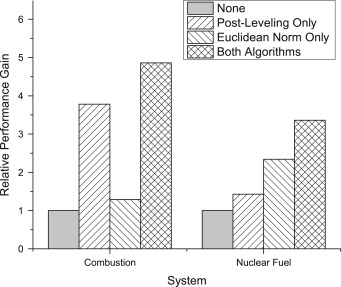
\includegraphics[width=0.65\textwidth]{figures/PEA_Gains}
%		\caption{Performance gains when employing post-levelling and Euclidean-norm algorithms \cite{Piro12a}.}
%		\label{fig:PEA_gains}
%	\end{figure}
%

%	\subsection{Temporal series estimate}
%	While in most cases levelling and post-levelling methods can provide initial assemblages close to the final assemblage, using the assemblage from a previous time step in multiphysics codes can often provide much closer estimates to the final assemblage. In time-dependent multiphysics simulations, this can result in significant performance gains as has been recently shown through the implementation of this strategy in {Thermochimica} \cite{Poschmann:2019aa}. These performance gains can be attributed to the fact that the convergence of the non-linear solver can be significantly accelerated by providing initial estimates close enough to the final assemblage. This temporal initialisation strategy has been illustrated in figure~\ref{fig:temp_init}
%	\begin{figure}
%		\centering
%		\begin{tikzpicture}[auto,
%    			block_center/.style ={rectangle, draw=black, thick, fill=white, text width=0.2\textwidth, text centered, minimum height=2em},
%    			block_side/.style ={rectangle, draw=black, thick, fill=white, text width=0.2\textwidth, text centered, minimum height=2em},
%			block_noborder/.style ={rectangle, draw=none, thick, fill=none, text width=0.2\textwidth, text centered, minimum height=0.5em},
%			block_small/.style ={rectangle, draw=none, thick, fill=none, text width=0.1\textwidth, text centered, minimum height=0.5em},
%			line/.style ={draw, thick, -stealth}]
%    			% Outlining the flowchart using the PGF/TikZ matrix funtion
%    			\matrix [column sep=0.15\textwidth,row sep=3em] {
%      				\node [block_center] (00) {Start at initial time}; & {} & {}\\
%      				\node [block_center] (10) {Levelling}; & {} & {}\\
%				\node [block_center,yshift=-1cm] (20) {Non-linear solver}; &  \node [block_side,yshift=-1cm] (21) {Save assemblage in memory}; & \node [block_side,yshift=-1cm] (22) {Reinitialise with saved assemblage};\\
%      				\node [block_side] (30) {Solution found}; & {} & {}\\
%    			};	% end matrix
%    			% connecting nodes with paths
%    			\begin{scope}[every path/.style=line]
%      				\path (00) edge (10);
%     				\path (10) edge (20);
%      				\path (20) edge node[block_noborder,anchor=east]{\footnotesize{Stop time reached}} (30);
%      				\path (20) edge (21);
%      				\path (21) edge node[block_noborder,anchor=south]{\footnotesize{Timestep}} (22);
%      				\path[-] (22.90) edge[bend right] node[block_noborder,anchor=west,shift={(0.75cm,0.25cm)}]{\footnotesize{Temporal reinitialisation failed}} (10);
%      				\path[-] (22) edge[bend right] (20);
%    			\end{scope}
% 		\end{tikzpicture}
%  		\caption{Illustration of the temporal series initialisation algorithm.}
%  		\label{fig:temp_init}
% 	\end{figure}
%
%	The details of the implementation of the temporal initialisation strategy in {Yellowjacket} have not yet been set in stone but, based on {Thermochimica} acceleration results obtained by Poschmann et al. \cite{Poschmann:2019aa} , a significant performance gain is foreseen which justifies the use of this strategy especially in coupled multiphysics problems where thermodynamic equilibrium calculations are impediment to significant performance gains. However, this might also lead to a drastic increase in memory requirement and a compromise must be made between  computing time gains and increased memory requirements.
%
%	\subsection{Boundary value estimate}
%	For the case where Gibbs energy minimisation is performed on a 2D/3D mesh, very good initial estimates can conceivably be provided to the non-linear solver by exploiting the results from the neighbouring solutions in space at the same time step. As an example, the final assemblage of element A on the finite element mesh shown in figure~\ref{fig:BV_Illustration} can be used as the initial assemblage for element B. This initialisation scheme relies on the principles of continuum between adjacent cells, i.e., if the mesh is sufficiently resolved, the difference between system potentials (temperature, pressure and chemical potentials) between two neighbouring cells must be small.
%	\begin{figure}[htbp]
%		\centering
%		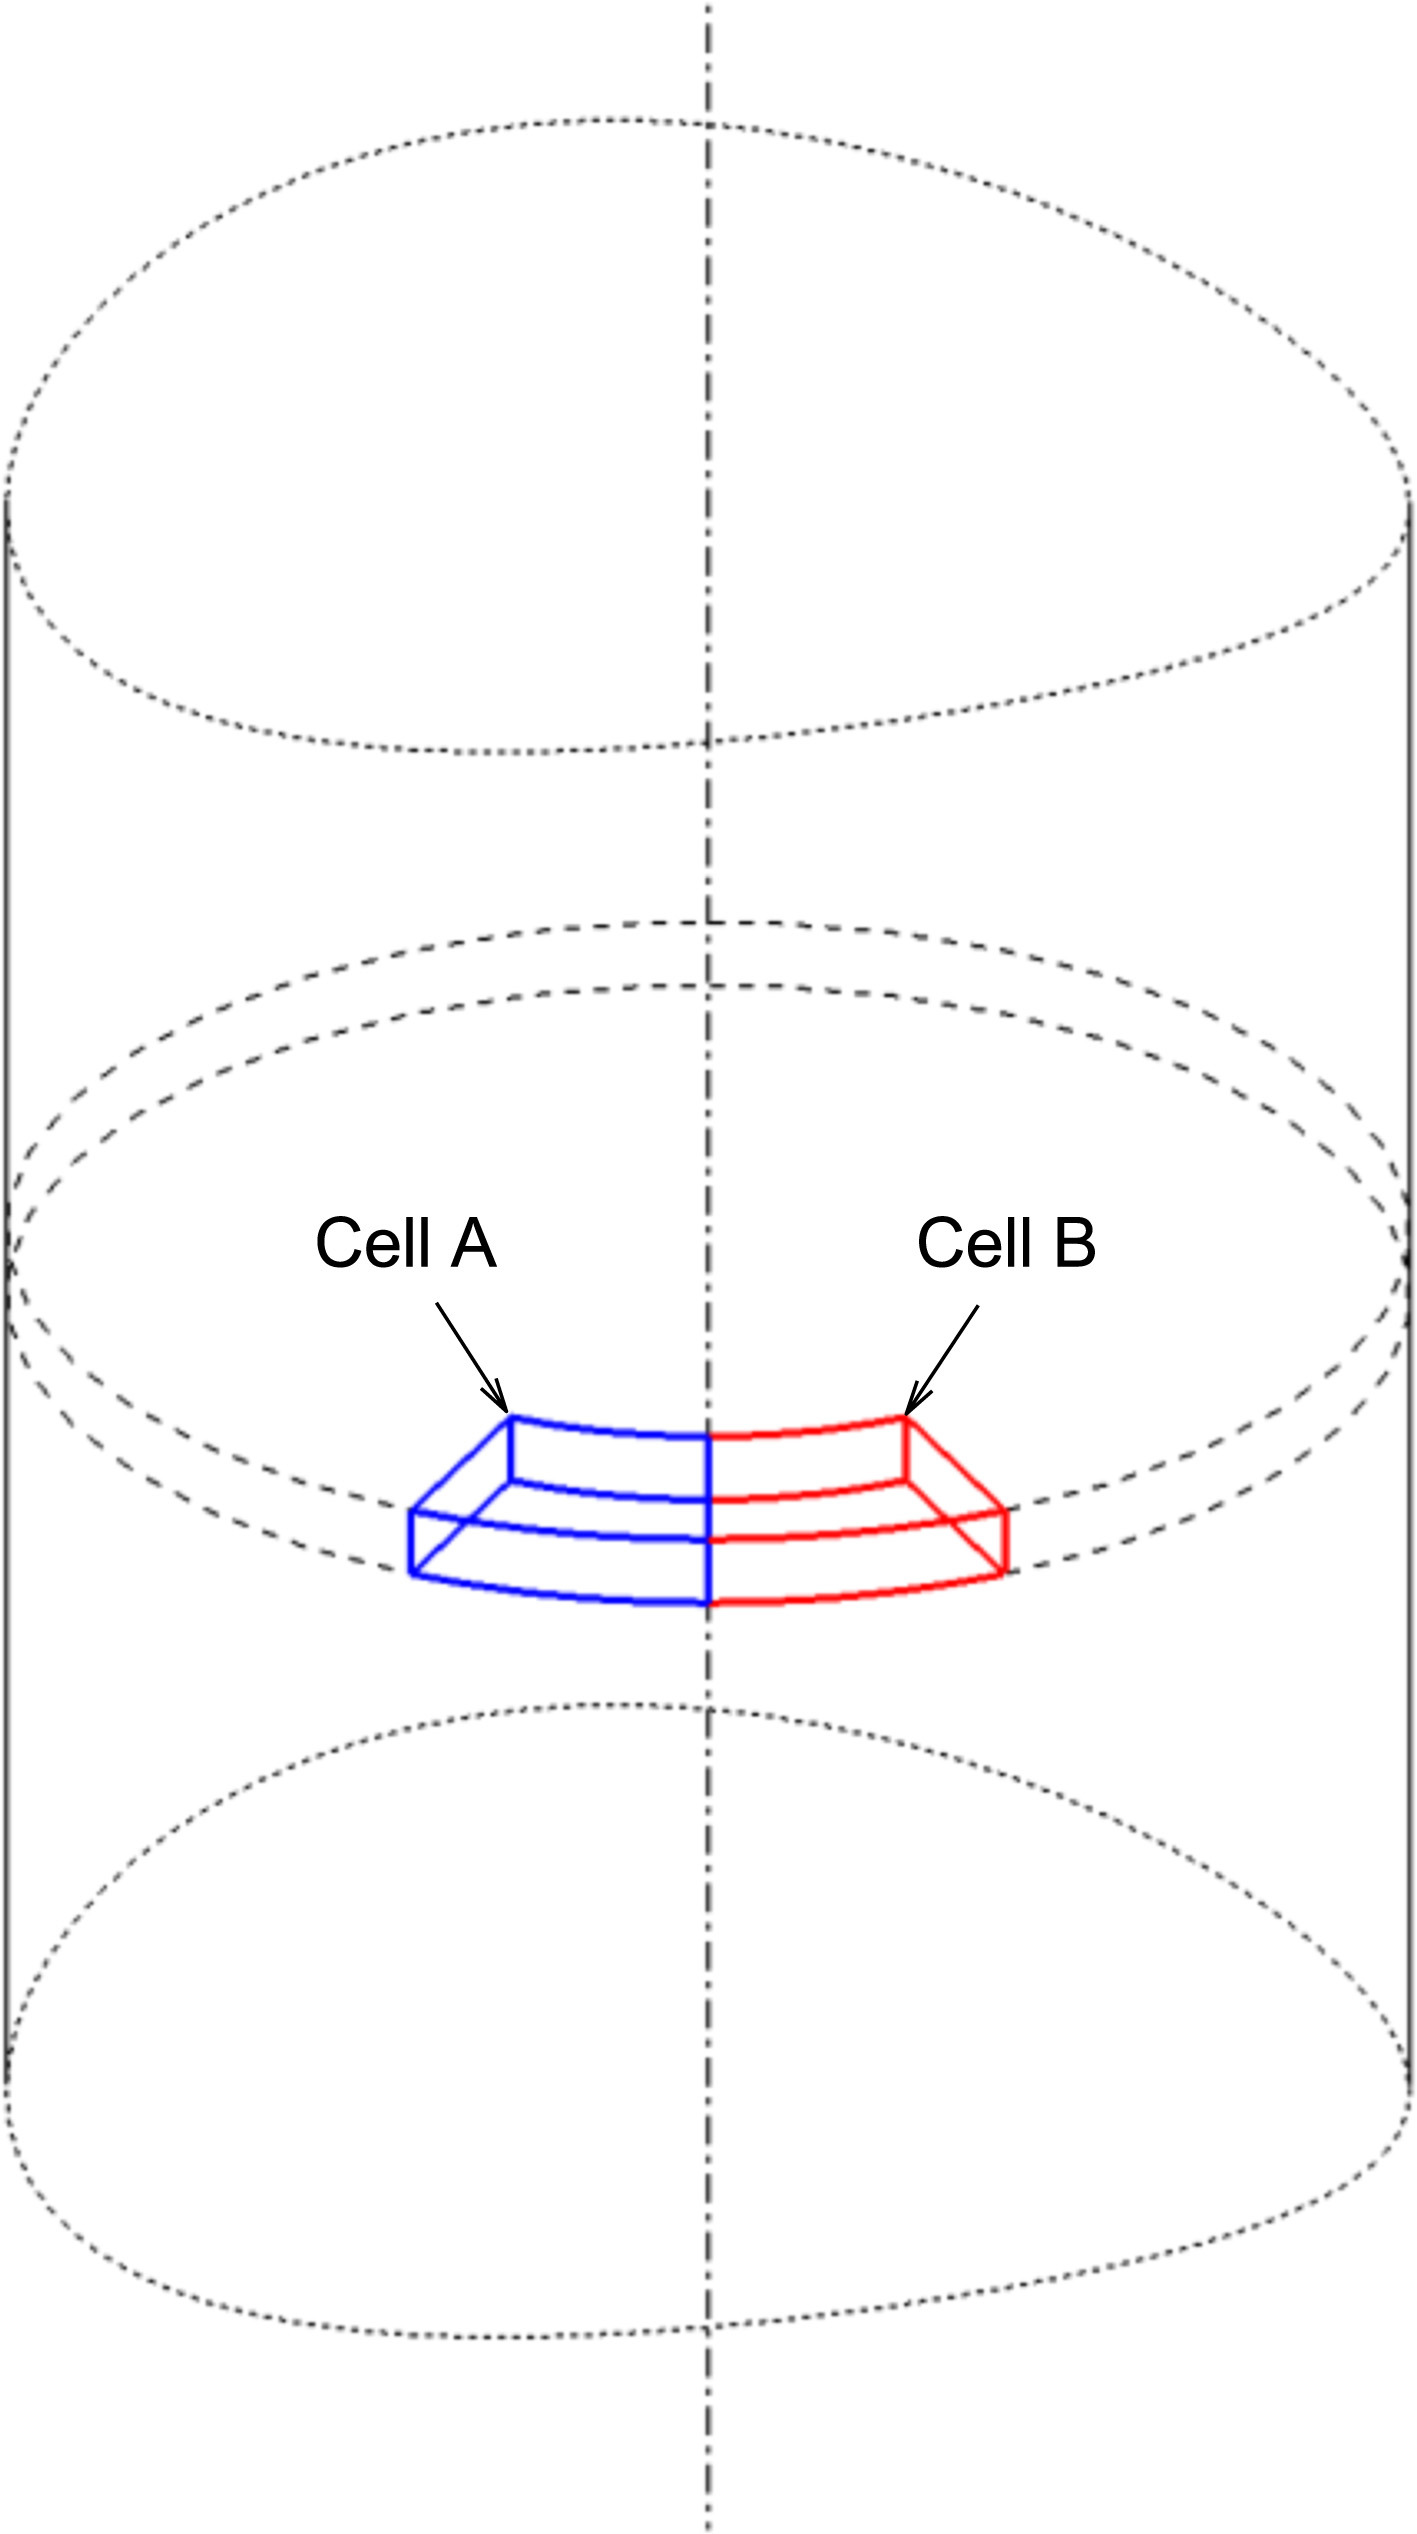
\includegraphics[width=0.35\textwidth]{figures/BV_FEM}
%		\caption{Illustration of the boundary value initialisation on a finite element mesh \cite{Piro17}.}
%		\label{fig:BV_Illustration}
%	\end{figure}
%
%	While this approach is well suited to simulations on finite element meshes and reduces the need to re-evaluate the estimated assemblage of stable phases, it might lead to a less than optimal estimate for elements close to a moving interface (for example, close to a melting boundary). Also, this approach does not lend itself well to parallel computing using MPI and thus might actually be ineffective for large problems where MPI can significantly speed up calculations. However, the approach is a potential avenue that can be explored but is not the primary focus.

\section{Non-linear solver}
	The linear solver can often provide estimates close to the final assemblage of the system and in certain circumstances, such as for systems with only pure 	stoichiometric species, it might be able to predict the equilibrium assemblage. However, almost always, further computations are required to arrive at the final assemblage especially in cases where the phases have more than one species with significant contribution to the Gibbs energy. This situation arises more often than not and a non-linear solver is required to handle the non-linearities arising from the logarithmic term in the compositional component of the chemical potentials.

	For the sake of completeness of the argument, the conditions for equilibrium are restated below:
	\begin{enumerate}
		\item The mass balance constraint must be satisfied.
		\item The Gibbs' phase rule must be satisfied.
		\item The integral Gibbs energy must be at a global minimum.
	\end{enumerate}

	The following subsidiary conditions arise from the constraints
	\begin{enumerate}[label=\Alph*.]
		\item The number of moles of any species must be positive.
		\item The sum of mole fractions must be one (inherent in the Gibbs energy method).
	\end{enumerate}
	
	\subsection{Numerical implementation}
	The system of non-linear equations can be solved using either the Newton-Raphson method. Newton-Raphson method depends on solving  equation~\eqref{eq:GEM_mat} and is an $\mathcal{O}(N^3)$ operation.
	An integral component of the solver is an appropriate line-search algorithm to determine how far the system should progress along the direction vectors. The functional norm of the Lagrangian is an effective choice to ensure convergence and is defined as \cite{Piro17}:
	\begin{equation}
	\begin{aligned}
		\|f\|^2 = &\sum_{j=1}^{C}\left(\sum_{\lambda=1}^{\Lambda} n_\lambda \sum_{i=1}^{N_\lambda} x_{i(\lambda)}\nu_{ij} + \sum_{\omega=1}^{\Omega}n_{\omega}\nu_{\omega,j} - b_j\right)^2 \\
		&+ \sum_{\lambda=1}^{\Lambda} \left(\sum_{i=1}^{N_\lambda} x_{i(\lambda)}\left\vert\mu_{i(\lambda)} - \sum_{j=1}^{C}\nu_{ij} \Gamma_j \right\vert \right)^2 + \sum_{\omega=1}^{\Omega}\left(g_\omega - \sum_{j=1}^{C}\nu_{\omega,j} \Gamma_j \right)^2
		\end{aligned}
	\end{equation}
	where the first term on the right represents the mass balance residuals, the second represents the absolute sum of chemical potential residuals of solution species and the third represents the chemical potential residuals of stoichiometric phases. By enforcing the Wolfe/Armijo condition \cite{Nocedal06}, a sufficient step length can be decided.

	Each iteration step in the minimisation problem involves approximately solving the subproblem
	\begin{equation}
		\min_\alpha f\left(\mathbf{x}^m + \alpha \mathbf{p}^m\right)
	\end{equation}
	where $\mathbf{x}^m$ is the best estimate at iteration $m$, $\mathbf{p}^m$ denotes the search direction vector and $\alpha$ represents the step size.

	The Wolfe conditions are a set of inequalities for performing inexact line search and provide an efficient way of computing an acceptable step length $\alpha$  that reduces the objective function sufficiently, rather than minimising the objective function over $\alpha \in \mathbb {R}^{+}$ exactly.

	A step length $\alpha^m$ is said to satisfy the Wolfe conditions, restricted to the direction $\mathbf{p}^m$, if the following two inequalities hold:
	\begin{equation}
		f\left(\mathbf{x}^m + \alpha^m \mathbf{p}^m\right) \leq f\left(\mathbf{x}^m \right) + c_1 \alpha^m \left(\mathbf{p}^m\right)^T \nabla f\left(\mathbf{x}^m \right)
	\end{equation}
	\begin{equation}
		- \left(\mathbf{p}^m\right)^T \nabla f\left(\mathbf{x}^m + \alpha^m \mathbf{p}^m\right) \leq - c_2 \left(\mathbf{p}^m\right)^T \nabla f\left(\mathbf{x}^m \right)
	\end{equation}
	with $0 < c_1 < c_2 < 1$. The first inequality, known as the Armijo condition ensures that the step length $\alpha^m$ decreases $f$ sufficiently, and the second inequality known as the curvature condition ensures that the slope has been reduced sufficiently. Together, the two inequalities provide upper and lower bounds for the step lengths \cite{Nocedal06}.

	\subsection{Adding/Removing phases}
		Updating the estimated assemblage plays a significant role in the convergence of thermodynamic solvers. Inadequate strategies for updating the assemblage might lead to inefficient global iterations (i.e., iterations in which changes are made to the system such as addition/removal of phases while the Newton iterations described above can be referred to as local iteration since they are aimed at finding the minimum of a problem with a fixed system) and might even prevent convergence. Though the number of phases that can be added into or removed from the system is constrained by the Gibbs' phase rule, proper care must be taken to ensure that any change to the system drives it towards convergence and not hold it back. To ensure that the phase assemblage updating does not result in undesired behaviour, the strategy proposed by Piro \cite{Piro17} will be adopted. This strategy has been illustrated in figure~\ref{fig:assemblage}

	\subsection{Convergence criterion}
	The convergence of the solver is tested in accordance with conditions for convergence described in chapter~\ref{chapter_3}. The relative error of the mass balance and Gibbs' criterion is calculated  and the solver converges when both of these are within the specified tolerance. In addition, it must be tested that the mole numbers are not negative for any species in the system. The charge neutrality constraint must also be respected.  To minimise the computational cost, it is also possible to test convergence only when the functional norm has been satisfied to a specified tolerance.

	Two issues that can prevent convergence are foreseen for a thermodynamic equilibrium solver. First, when the objective function has multiple roots, for example due to miscibility gap, and second when the slope of the objective function is extremely small or zero. These two issues can result in non-real numbers or divergence and possible failure of the iterative solver.

	The numerical dampening through Wolfe/Armijo conditions and the use of levelling as an initialisation method can help in avoiding the ill-behaviour and promotes numerical stability and enhances performance characteristics. The proposed algorithm of the thermodynamic solver with both local and global iterations has been presented in fig.~\ref{fig:gem_illus}

\newgeometry{margin=1cm}
\begin{landscape}
\thispagestyle{empty}

		\begin{figure}
		\centering
		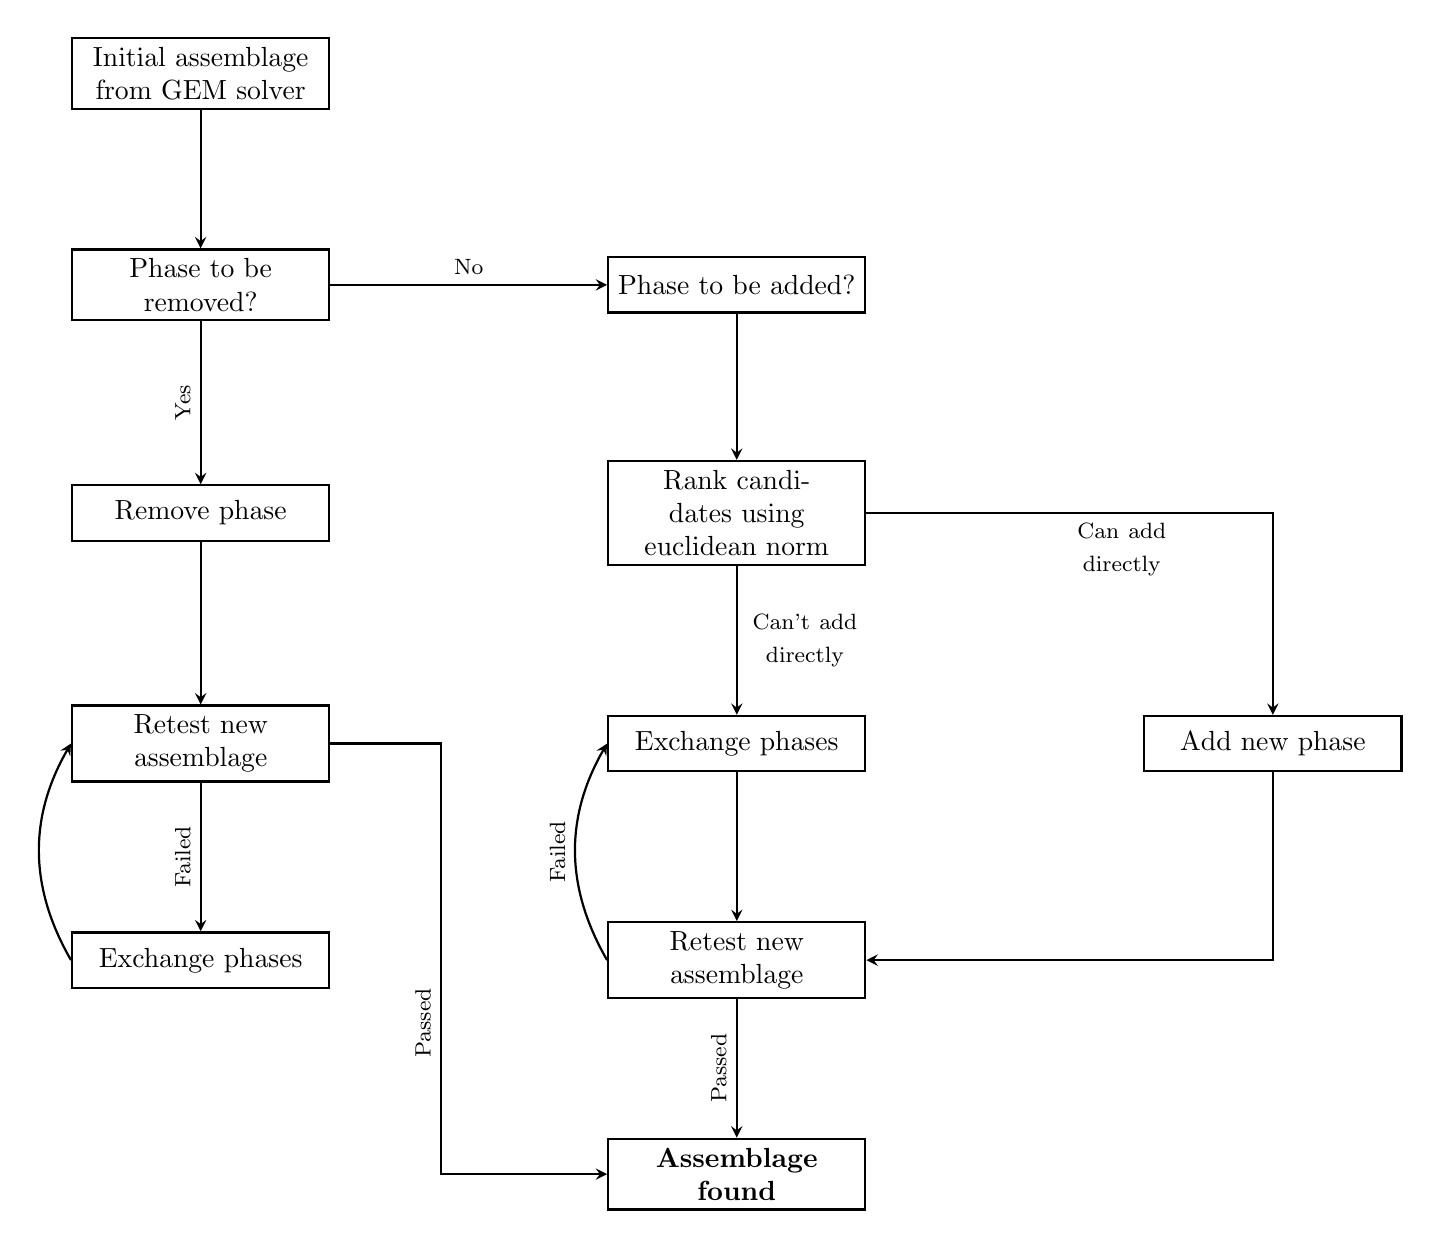
\begin{tikzpicture}[auto,
    			block_center/.style ={rectangle, draw=black, thick, fill=white, text width=0.25\textwidth, text centered, minimum height=2em},
    			block_side/.style ={rectangle, draw=black, thick, fill=white, text width=0.15\textwidth, text centered, minimum height=2em},
			block_noborder/.style ={rectangle, draw=none, thick, fill=none, text width=0.15\textwidth, text centered, minimum height=0.5em},
			block_small/.style ={rectangle, draw=none, thick, fill=none, text width=0.1\textwidth, text centered, minimum height=0.5em},
			line/.style ={draw, thick, -stealth}]
    			% Outlining the flowchart using the PGF/TikZ matrix funtion
    			\matrix [column sep=10em,row sep=5em] {
      				\node [block_center] (00) {Initial assemblage from GEM solver}; & {} \\
      				\node [block_center] (10) {Phase to be removed?}; & \node [block_center] (11) {Phase to be added?}; \\
				\node [block_center] (20) {Remove phase}; & \node [block_center] (21) {Rank candidates using euclidean norm}; & {}\\
				\node [block_center] (30) {Retest new assemblage}; & \node [block_center] (31) {Exchange phases}; & \node [block_center] (32) {Add new phase};\\
				\node [block_center] (40) {Exchange phases}; & \node [block_center] (41) {Retest new assemblage}; & {} \\
				{} & \node [block_center] (51) {\textbf{Assemblage found}}; & {}\\
    			};	% end matrix
    			% connecting nodes with paths
    			\begin{scope}[every path/.style=line]
      				\path (00) edge (10);
     				\path (10) edge node[block_noborder,rotate=90,anchor=south]{\footnotesize{Yes}} (20);
				\path (10) edge node[block_noborder]{\footnotesize{No}} (11);
				\path (20) edge (30);
				\path (30) edge node[block_noborder,rotate=90,anchor=south]{\footnotesize{Failed}} (40);
%				\path (30.360)[-] edge node[block_noborder]{\footnotesize{Passed}} (51.180);
				\path (30.360) -- +(4em,0) |- node[block_noborder,rotate=90,anchor=south west,xshift=2.5em]{\footnotesize{Passed}} (51.180);
				\path[-] (40.180) edge[bend left] (30.180);
				\path (11) edge (21);
				\path (21) edge node[block_noborder,anchor=west,xshift=-0.5em]{\footnotesize{Can't add directly}} (31);
				\path (21.360) -| node[block_noborder,anchor=north east,xshift=-2.5em]{\footnotesize{Can add directly}} (32.90);
				\path (31) edge (41);
				\path (32.270) |- (41.360);
				\path[-] (41.180) edge[bend left] node[block_noborder,rotate=90,anchor=south]{\footnotesize{Failed}}(31.180);
				\path (41) edge node[block_noborder,rotate=90,anchor=south]{\footnotesize{Passed}}(51);
			\end{scope}
 		\end{tikzpicture}
  		\caption{Illustration of the proposed methodology for updating the phase assemblage. Adapted from Piro \cite{Piro17}.}
  		\label{fig:assemblage}
	\end{figure}

\end{landscape}
\restoregeometry

\newgeometry{margin=1cm}
\begin{landscape}
\thispagestyle{empty}

	\begin{figure}
		\centering
		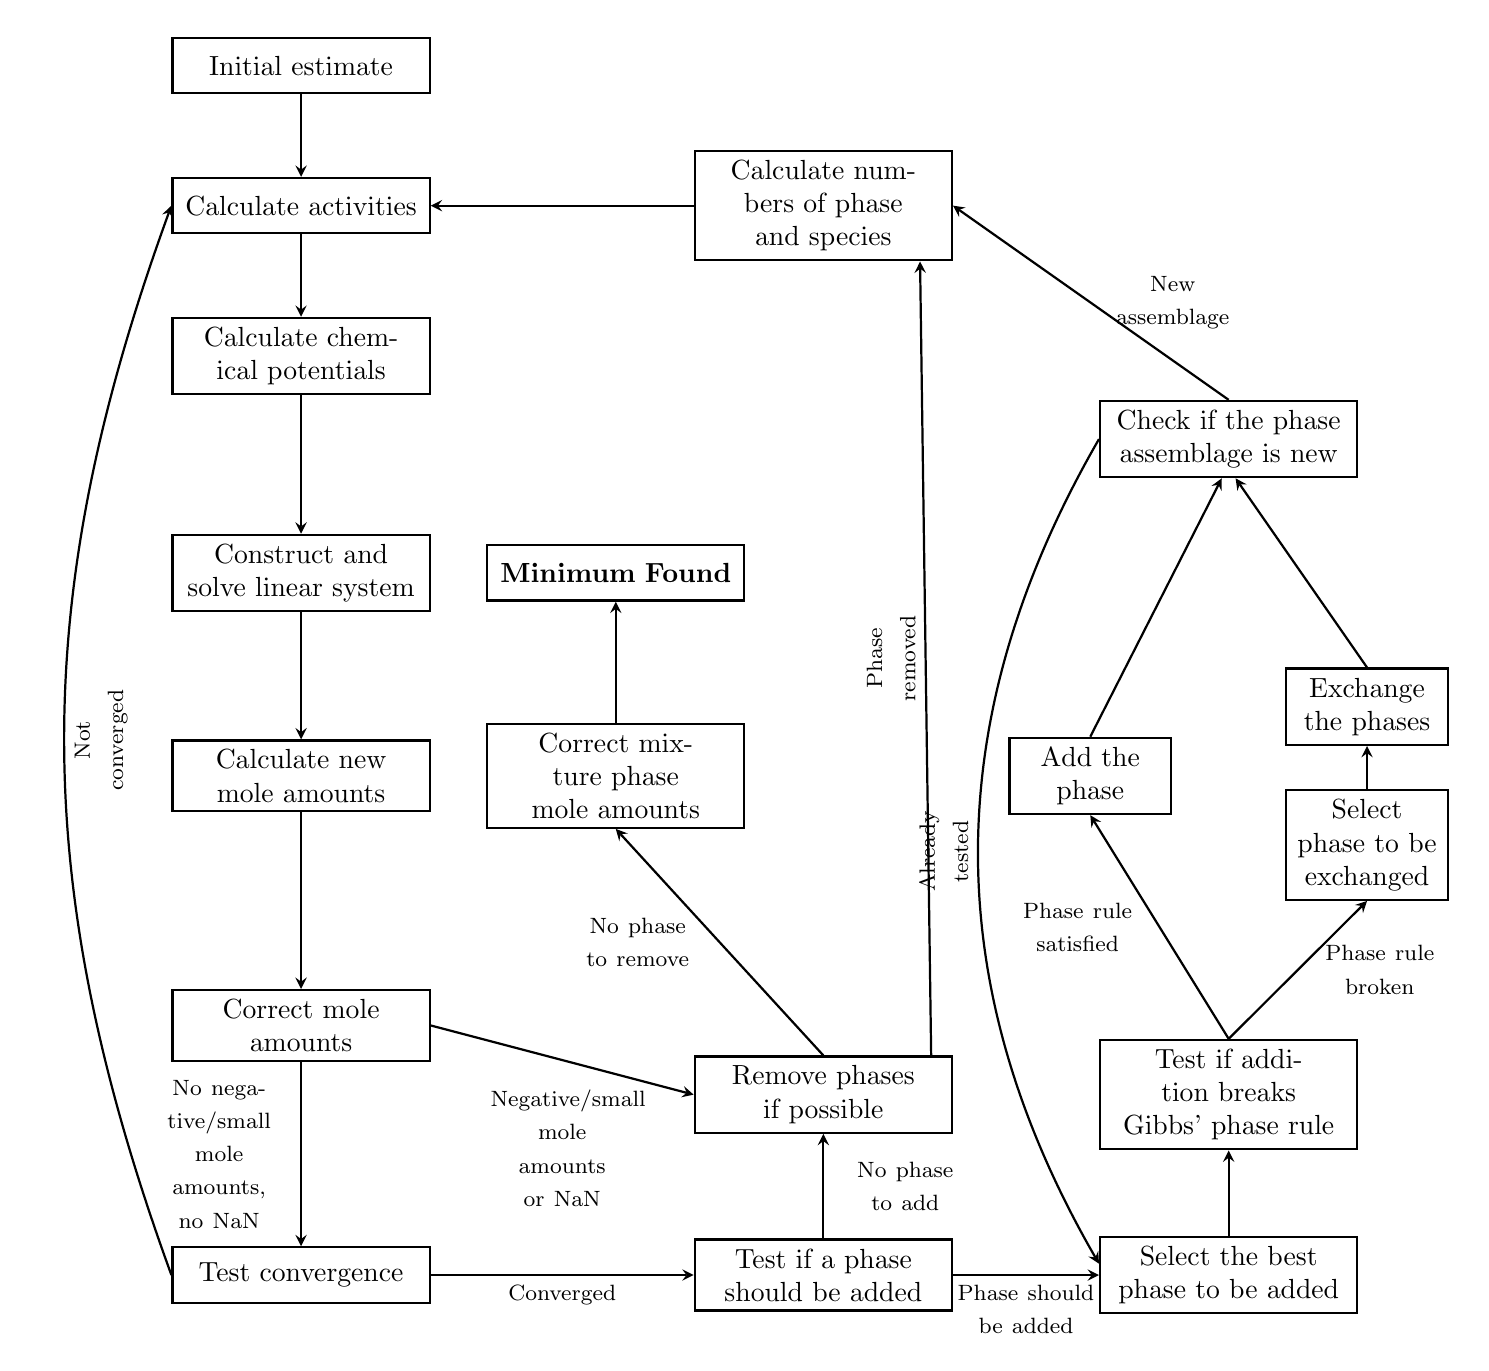
\begin{tikzpicture}[auto,
    			block_center/.style ={rectangle, draw=black, thick, fill=white, text width=0.25\textwidth, text centered, minimum height=2em},
    			block_side/.style ={rectangle, draw=black, thick, fill=white, text width=0.15\textwidth, text centered, minimum height=2em},
			block_noborder/.style ={rectangle, draw=none, thick, fill=none, text width=0.15\textwidth, text centered, minimum height=0.5em},
			block_small/.style ={rectangle, draw=none, thick, fill=none, text width=0.1\textwidth, text centered, minimum height=0.5em},
			line/.style ={draw, thick, -stealth}]
    			% Outlining the flowchart using the PGF/TikZ matrix funtion
    			\matrix [column sep=2em,row sep=2em] {
      				\node [block_center] (00) {Initial estimate}; & {} & {} \\
      				\node [block_center] (10) {Calculate activities}; & \node [block_center] (11) {Calculate numbers of phase and species}; & {}\\
				\node [block_center] (20) {Calculate chemical potentials}; & {} & \node [block_center,yshift=-3em] (22) {Check if the phase assemblage is new};\\
				\node [block_center] (30) {Construct and solve linear system}; & \node [block_center,xshift=-7.5em] (31) {\textbf{Minimum Found}}; & {}\\
				\node [block_center] (40) {Calculate new mole amounts}; & \node [block_center,xshift=-7.5em] (41) {Correct mixture phase mole amounts}; & \node [block_side,xshift=-5em] (42a) {Add the phase};  \node [block_side,xshift=5em,yshift=-2.5em] (42b) {Select phase to be exchanged}; \node [block_side,xshift=5em,yshift=2.5em] (42c) {Exchange the phases};\\
				\node [block_center,yshift=-2.5em] (50) {Correct mole amounts}; & \node [block_center,yshift=-5em] (51) {Remove phases if possible}; & \node [block_center,yshift=-5em] (52) {Test if addition breaks Gibbs' phase rule};\\
				\node [block_center,yshift=-2.5em] (60) {Test convergence}; &  \node [block_center,yshift=-2.5em] (61) {Test if a phase should be added}; & \node [block_center,yshift=-2.5em] (62) {Select the best phase to be added};\\
    			};	% end matrix
    			% connecting nodes with paths
    			\begin{scope}[every path/.style=line]
      				\path (00) edge (10);
     				\path (10) edge (20);
				\path (20) edge (30);
				\path (30) edge (40);
				\path (40) edge (50);
				\path (50) edge node[block_noborder,anchor=east]{\footnotesize{No negative/small mole amounts, no NaN}} (60);
				\path (60) edge node[block_noborder,anchor=north]{\footnotesize{Converged}} (61);
				\path (61) edge node[block_noborder,anchor=north]{\footnotesize{Phase should be added}} (62);
				\path (62) edge (52);
				\path (61) edge node[block_noborder,anchor=west]{\footnotesize{No phase to add}} (51);
				\path[-] (51.90) edge node[block_noborder,anchor=east]{\footnotesize{No phase to remove}} (41.270);
				\path (41) edge  (31);
				\path[-] (51.20) edge node[block_noborder,anchor=south,rotate=90]{\footnotesize{Phase  removed}}(11.330);
				\path[-] (60.180) edge[bend left=20] node[block_noborder,anchor=north,rotate=90]{\footnotesize{Not converged}} (10.180);
				\path[-] (50.360) edge node[block_noborder,anchor=north,yshift=-0.25cm]{\footnotesize{Negative/small mole amounts or NaN}} (51.180);
				\path[-] (52.90) edge node[block_noborder,anchor=east]{\footnotesize{Phase rule satisfied}}(42a.270);
				\path[-] (52.90) edge node[block_noborder,anchor=west]{\footnotesize{Phase rule broken}}(42b.270);
				\path (42b) edge  (42c);
				\path[-] (42c.90) edge  (22.280);
				\path[-] (42a.90) edge  (22.260);
				\path[-] (22.90) edge node[block_noborder,anchor=west]{\footnotesize{New assemblage}}(11.360);
				\path (11) edge  (10);
				\path[-] (22.180) edge[bend right=30] node[block_noborder,anchor=south,rotate=90]{\footnotesize{Already tested}} (62.175);
			\end{scope}
 		\end{tikzpicture}
  		\caption{Illustration of the proposed Gibbs energy minimisation algorithm}
  		\label{fig:gem_illus}
	\end{figure}

\end{landscape}
\restoregeometry

%==============================================================================================================================
%														Global Optimisation
%==============================================================================================================================
\section{Global Optimisation}
%Ensuring that the global minimum of Gibbs energy is correctly calculated requires that the driving force of all metastable phases be positive. As described in section~\ref{sec:global_opt_intro}, computing the minimum driving force of a thermodynamic system requires solving a non-convex constrained optimisation problem. 
%
%	The computation of thermodynamic equilibrium, as discussed in sec.~\ref{sec:opt_theory}, is a global optimisation problem where the focus is on systems that can attain equilibrium state under conditions of constant temperature and pressure, where the global minimum value of the Gibbs energy describes the true equilibrium state. The problem can be stated as follows \cite{Floudas99}:
%	\begin{objective}
%	Given $C$ components participating in up to $\Phi$ potential phases under isothermal and isobaric conditions find the mole vector $\mathbf{n}$ that minimises the value of the Gibbs energy while also satisfying the appropriate material balance constraints.
%	\end{objective}
%
%	\begin{constraint}
%		The mole fraction of a species in phase $\lambda$, $x_{i(\lambda)}$, must satisfy the following linear equality and inequality constraints
%		\begin{equation}
%		\sum_{i=1}^{N_\lambda} x_{i(\lambda)} = 1 \mspace{30mu}x_{i(\lambda)} > 0\mspace{30mu} \forall i
%		\end{equation}
%	\end{constraint}
%
%The component set is represented by the index set $C = \{i\}$ and the elements that constitute these components are given by $E  = \{e\}$. The set of phases is denoted by $\Phi = \{k\}$ where it is composed of solution and stoichiometric phases, labelled $\Lambda$ and $\Omega$ respectively, so that $\Phi \equiv \Lambda\cup \Omega$.

	As described in section~\ref{sec:global_opt_intro}, computing the minimum driving force of a thermodynamic system requires solving a non-convex constrained optimisation problem. The conditions for thermodynamic equilibrium discussed in section~\ref{sec:eqb_theory} require that the chemical potentials of all the species must lie on or above the Gibbs plane, which passes through the element potentials $\Gamma_j$. Thus metastable phases must lie above the Gibbs plane and the difference between the Gibbs plane and the plane tangent to a metastable phase is referred to as the \emph{driving force} \cite{Lukas07} or \emph{tangent plane distance function} \cite{Lukas07,Zhang11}. The driving force for phase $\phi$ is represented by $\Delta G_{\phi}$ and is computed as \cite{Piro16}:
	\begin{equation}\label{eq:drivingforce}
        		\Delta G_{\phi}= \min_{\lambda} \sum_{i=1}^{N_{\lambda}}x_{i} \left (\mu_{i} - \sum_{j=1}^C \nu_{ij}\Gamma_j \right ),
    	\end{equation}
	which is subject to conservation of mass and the following linear equality and inequality constraints:
	\begin{align}
		\sum_{i=1}^{N_\phi} x_i = 1, \; x_i > 0, \; \forall i \in \phi.
	\end{align}
	The sufficient condition for equilibrium requires that the driving force $\Delta G_{\phi}$ computed with equation~\eqref{eq:drivingforce} is positive for all phases believed to be metastable and zero for all the stable phases. According to Hillert \cite{Hillert81}, the driving force of metastable phases can be evaluated at each iteration to determine whether or not it should be added into the system. However, this function can be non-convex and requires the evaluation of a global minimum. Though the open literature on computing these methods appears rather exhaustive, few authors have discussed generalised global minimisation schemes for the phase equilibria problem. The majority of articles focus either on relatively small systems, such as liquid-vapour equilibria, or are aimed at only a handful of calculations. Some notable exceptions to this include those of Hillert \cite{HILLERT198131}, Lukas \textit{et al.}\cite{LUKAS1982229}, Sundman \cite{Sundman15}, Piro and Simunovic \cite{Piro16}, and Otis \textit{et al.} \cite{Otis:2017ab}. Since both the robustness and computational efficiency of {\GEM} are of concern, a number of global optimisation methods were tested through a set of carefully constructed test problems representative of some common scenarios in equilibrium thermodynamics. Though no global optimisation method can guarantee the ability to find the true global minimum, sufficient confidence can be achieved for the problem under consideration under well-defined parameters.
	
	\subsection{Test Problems} \label{sec:test_global}
	To objectively test the reliability and performance of various global optimisation algorithms, the methods must be benchmarked against a set of test problems representative of the requirements from the solver. While most of the open  literature focusses on a single problem and tries to optimise the algorithm for the problem, such an approach is not ideal for the development of {\GEM}. Instead the focus here has been to select an algorithm that can work reasonably well for wide variety of problems with a large number of components. The reasoning behind such an approach is that a wide variety of excess mixing models are encountered in computational thermodynamics applied to nuclear materials. To test the algorithms under consideration, eight test cases representing different thermodynamic models and system sizes, and are summarised in table~\ref{tab:test_cases}.
	\begin{table}[htbp]
		\centering
	   	\caption{Summary of test cases used for comparing global optimisation algorithms.}
	   	\begin{tabular}{@{} lcp{0.82\linewidth} @{}} % Column formatting, @{} suppresses leading/trailing space
	      		\toprule
	      		\textbf{Label}	& \textbf{Size}		& \textbf{Problem Description} \\
	      		\midrule
	      		A			& 2					& Fictive binary system with a miscibility gap and a stoichiometric phase from Piro and Simunovic \cite{Piro16}.\\
	      		B			& 2					& \ce{Pd-Rh} binary system with a shallow FCC miscibility gap phase from Kaye \textit {et al.} \cite{Kaye07}.\\
	      		C			& 2					& Fictive binary system with three convex phases with one phase having a negative driving force from Piro and Simunovic \cite{Piro16}. \\
	      		D			& 3					& \ce{Pu-U-O} ternary system from Gu\'{e}neau \textit{et al.} \cite{Gueneau11} containing an ideal gas phase, a non-ideal liquid phase, many stoichiometric phases and a \ce{(U$_y$ Pu$_{1-y}$)O$_{2\pm x}$} fluorite phase. Involves a multi-sublattice model and a charge balance constraint.\\
	      		E			& 3					& \ce{Al-Cr-Co} ternary system used as reference problem by Otis \textit {et al.} \cite{Otis:2017ab}. \\
	      		F			& 5					& Hexagonal closed packing (HCP) phase in the quinary system containing noble metal fission products \ce{Mo-Pd-Tc-Ru-Rh} from Kaye \textit {et al.} \cite{Kaye07}.\\
	      		G			& 10					& \multirow{2}{=}{Fictive high-dimensional systems with minefield of miscibility gaps based on Piro and Simunovic \cite{Piro16}.}\\
	      		H			& 30					& \\
	      \bottomrule
	   \end{tabular}
	   \label{tab:test_cases}
	\end{table}
	
	\begin{enumerate}
	\item	\emph{Problem A}\\
		A fictive binary  \ce{A-B} system based on Piro and Simunovic \cite{Piro16} has been considered as the first test problem. As shown previously in section~\ref{sec:global_opt_intro}, it consists of solution phase $\alpha$ and a stoichiometric phase \ce{A3B2} which can possibly coexist and while the stoichiometric phase \ce{A3B2} and solution phase $\alpha$ are initially predicted to be stable, as represented by the dashed tangent line in figure~\ref{fig:testA}, they are in fact metastable and a miscibility gap would yield a lower value of the integral Gibbs energy of the system, $G_\text{sys}$. The $\alpha$ phase is represented by a substitutional solution model with the reference Gibbs energies of the components being $g_{\ce{A}}^\circ = -100 $ \si{\joule \per \mole}, $g_{\ce{B}}^\circ = -300$ \si{\joule \per \mole} and the excess energy given by $g_{\alpha}^\text{ex} = 21000 x_{\ce{A}} x_{\ce{B}} + 7000 x_{\ce{A}} x_{\ce{B}}^2$. The temperature of the system was fixed at $T = 1000$ \si{\kelvin} and the pressure at $P=1$ \si{\atmosphere}.
		\begin{figure}[htbp]			
			\centering
			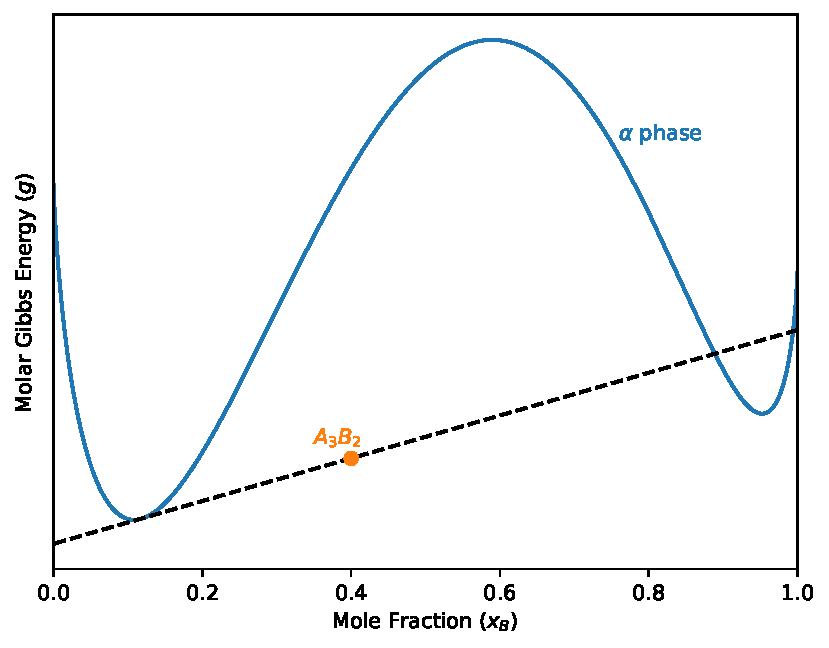
\includegraphics[width=0.6\textwidth]{figures/chapter-6/System_AB.pdf}
			\caption[Global optimisation test problem A: Fictive system with miscibility gap showing a possible false positive from thermodynamic equilibrium solver.]{Fictive system with miscibility gap showing a possible false positive from thermodynamic equilibrium solver.}
			\label{fig:testA}
		\end{figure}
 
	
	\item	\emph{Problem B}\\
		The binary  \ce{Pd-Rh} system from Kaye \textit{et al.} \cite{Kaye07} has been selected as the second test problem. It consists of a shallow miscibility gap in the FCC phase which is assumed to be properly identified by the solver but the global optimisation algorithm must confirm that the driving force, $\Delta G_\text{FCC}$, of the miscibility gap phase is indeed zero. The phase is represented by a substitutional solution model with the reference Gibbs energies of the components being $g_{\ce{Pd}}^\circ = -16480 + 9.02T$ \si{\joule \per \mole}, $g_{\ce{Rh}}^\circ = -26568 + 11.88 T$ \si{\joule \per \mole} and the excess energy given by $g_\text{FCC}^\text{ex} = x_{\ce{Pd}}x_{\ce{Rh}} \left(21247 + 2199 x_{\ce{Rh}} - (2.74 - 0.56x_{\ce{Rh}})T\right)$. The temperature of the system was fixed at $T = 1100$ \si{\kelvin} and the pressure at $P=1$ \si{\atmosphere}.
		\begin{figure}[htbp]			
			\centering
			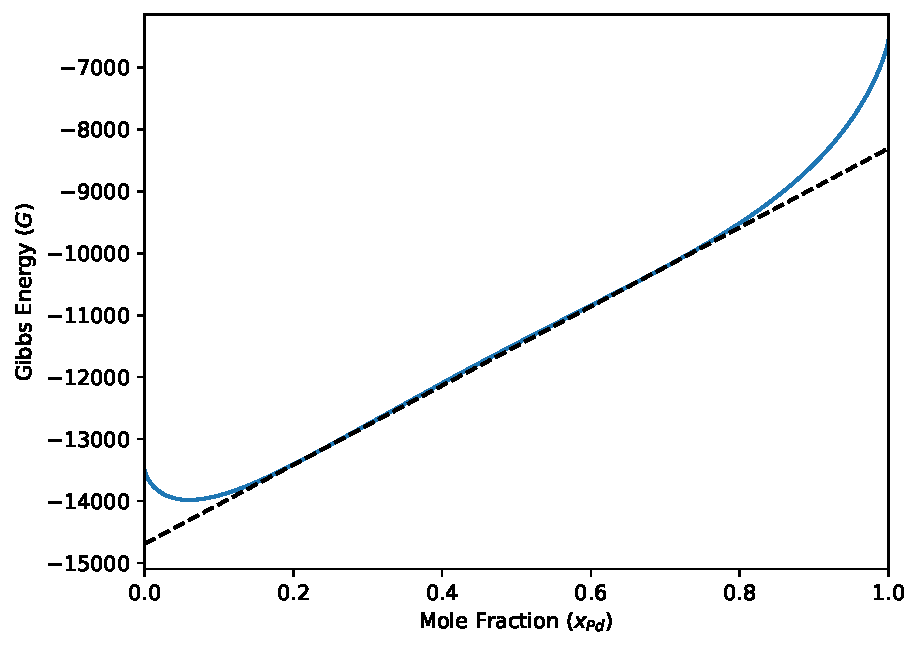
\includegraphics[width=0.675\textwidth]{figures/chapter-6/System_PdRh.pdf}
			\caption[Global optimisation test problem B: FCC phase miscibility gap in \ce{Pd-Rh} binary system.]{FCC phase miscibility gap in \ce{Pd-Rh} binary system from Kaye \textit{et al.} \cite{Kaye07} shows a correctly identified miscibility gap which must be verified by the global optimisation algorithm.}
			\label{fig:testB}
		\end{figure}

	\item	\emph{Problem C}\\
		Another fictive binary system, from Piro and Simunovic \cite{Piro16}, with components \ce{C-D} can have three possible solution phases, the $\delta$ phase as shown in figure~\ref{fig:testC}. At  temperature  $T = 1100$ \si{\kelvin}, pressure $P=1$ \si{\atmosphere} and composition $x_{\ce{D}} = 0.6$, the $\delta$ phase is believed to be metastable but one must confirm that the combination of $\beta$ and $\gamma$ is most stable or if a different combination is more stable. However, it can be seen that inserting the $\delta$ phase into the system and replacing one of the other two phases would yield a lower value of the integral Gibbs energy of the system, $G_\text{sys}$. For this system, $g_{\ce{C}(\beta)}^\circ = 0$ \si{\joule \per \mole}, $g_{\ce{D}(\beta)}^\circ = 12471$ \si{\joule \per \mole}, $g_{\ce{C}(\gamma)}^\circ = 16628$ \si{\joule \per \mole}, $g_{\ce{D}(\gamma)}^\circ = 4157$ \si{\joule \per \mole}, $g_{\ce{C}(\delta)}^\circ = 26604$ \si{\joule \per \mole} and $g_{\ce{D}(\delta)}^\circ = 33256$ \si{\joule \per \mole}. The molar Gibbs energies of mixing are $g_{\beta}^\text{ex} = 41570 x_{\ce{C}} x_{\ce{D}} - 58198 x_{\ce{C}}x_{\ce{D}}^2$, $g_{\gamma}^\text{ex} = -5238 x_{\ce{C}} x_{\ce{D}}$ and $g_{\delta}^\text{ex} = -59445 x_{\ce{C}} x_{\ce{D}} - 74826 x_{\ce{C}}x_{\ce{D}}^2$.
		\begin{figure}[htbp]
			\centering
			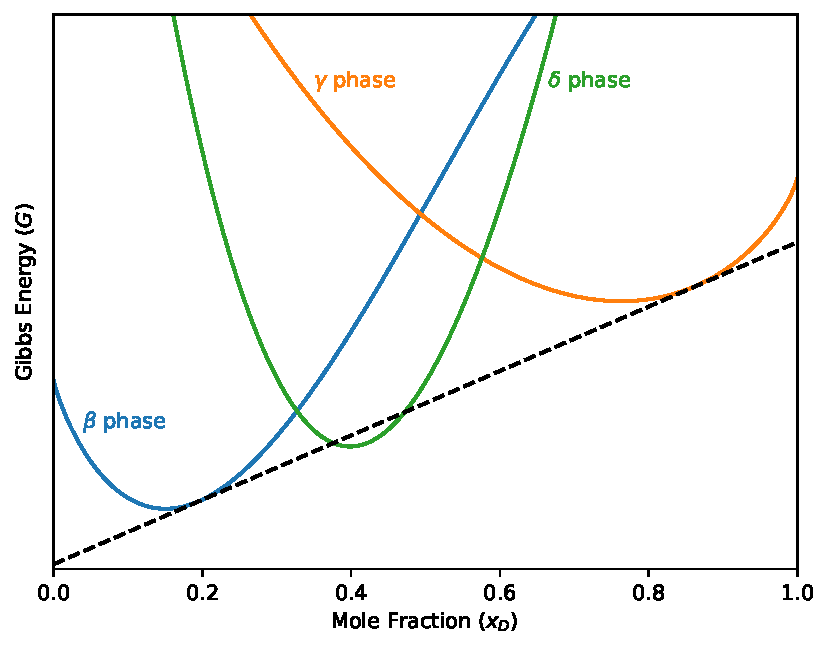
\includegraphics[width=0.6\textwidth]{figures/chapter-6/System_CD.pdf}
			\caption[Global optimisation test problem C: Fictive system with three phases showing a false positive from thermodynamic equilibrium solver wherein a wrong phase is believed to be present at equilibrium.]{Fictive system with three phases showing a false positive from thermodynamic equilibrium solver wherein a wrong phase is believed to be present at equilibrium.}
			\label{fig:testC}
		\end{figure}
	
	\item	\emph{Problem D}\\
		Mixed oxide fuel (MOX) is a nuclear fuel which is manufactured by mixing plutonium recovered from used reactor fuel with depleted uranium and the \ce{Pu-U-O} ternary system from Gu\'{e}neau \textit{et al.} \cite{Gueneau11} has been selected as a test problem. The thermodynamic assessment of the system contains an ideal gas, a non-ideal liquid,  and a \ce{(U_y Pu_{1-y})O$_{2\pm x}$} fluorite phase modelled using CEF with three sublattices and is an ionic phases where the first sublattice contains actinoid cations and the second and third sublattices contain oxygen anions mixing with vacancies. The global optimisation algorithm must respect the charge neutrality constraint thus distinguishing this problem from others. The system composition, as in \cite{Piro16}, is \SI{0.93}{\mole} of \ce{U}, \SI{0.07}{\mole} of \ce{Pu} and \SI{2}{\mole} of \ce{O} maintained at temperature $T = 1000$ \si{\kelvin} and hydrostatic pressure $P=1$ \si{\atmosphere}. The global optimisation algorithm must verify that the \ce{(U_y Pu_{1-y})O$_{2\pm x}$} fluorite phase is only stable phase at equilibrium.
		
	\item	\emph{Problem E}\\
		Otis \textit{et al.} \cite{Otis:2017ab} demonstrated that for the \ce{Al-Co-Cr} ternary system modelled by Liu \textit{et al.} \cite{Liu:2015aa} poses a challenge to thermodynamic equilibrium codes. In particular, it was shown that at temperature $T = 1523$  \si{\kelvin}, a ternary miscibility gap can be ignored when considering the metastable BCC phase only. The phase was modelled with a three-sublattice CEF model with the elements mixing on the first and second sublattices. Considering the challenges posed by the BCC phase in the system, the system was selected as a test problem with the system containing \SI{0.5}{\mole} of \ce{Al}, \SI{0.2}{\mole} of \ce{Co} and \SI{0.3}{\mole} of \ce{Cr} at $T = 1000$ \si{\kelvin} and $P=1$ \si{\atmosphere}. The global optimisation algorithm must identify the existence of a miscibility gap.
		\begin{figure}[htbp]
			\centering
			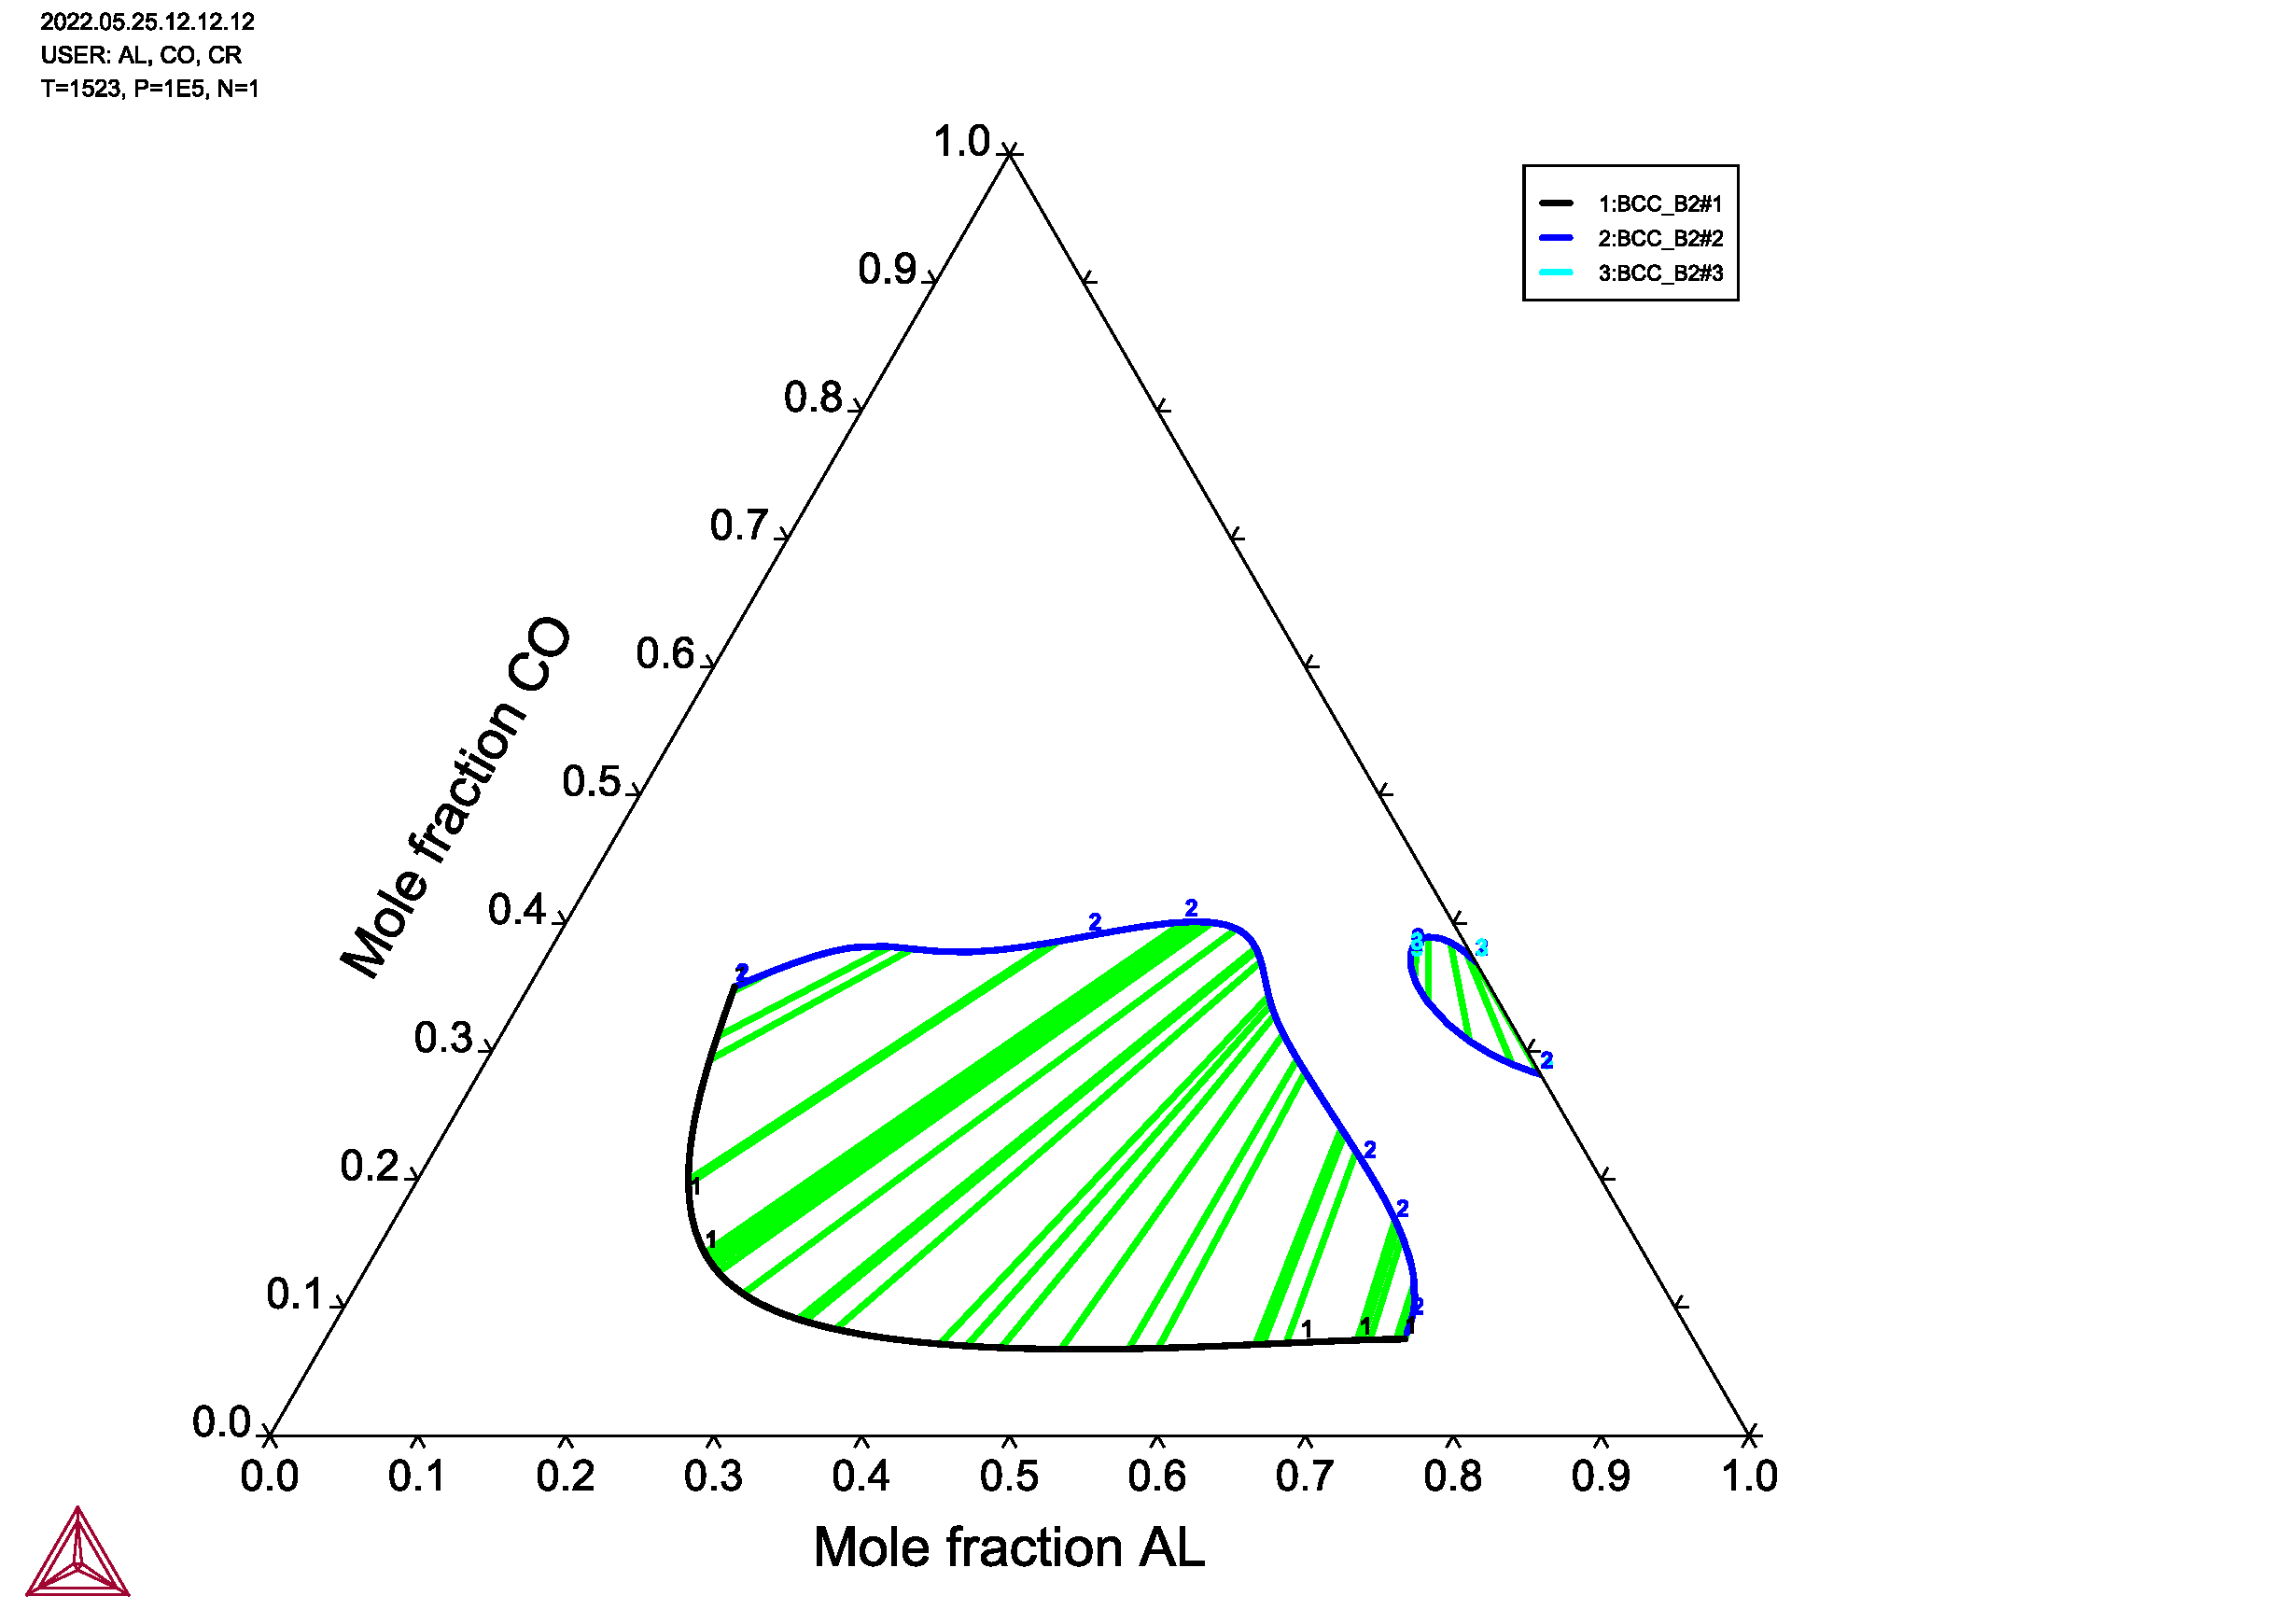
\includegraphics[width=0.6\textwidth]{figures/chapter-6/System_AlCoCr.pdf}
			\caption[Global optimisation test problem E: BCC phase \ce{Al-Co-Cr} ternary system with the miscibility gap.]{\ce{Al-Co-Cr} phase diagram calculated with Thermo-Calc version 2018b with an increased point density. With only BCC phase enabled, the existence of the miscibility gaps is shown in the central portion but as shown by Otis \textit{et al.} \cite{Otis:2017ab}, the miscibility gap is lost using the default Thermo-Calc parameters.}
			\label{fig:testE}
		\end{figure} 
	
	\item	\emph{Problem F}\\
		The quinary \ce{Mo-Pd-Tc-Ru-Rh} system from Kaye \textit {et al.} \cite{Kaye07} is considered as the sixth test problem for comparing global optimisation algorithms. The system is relevant to nuclear reactor accident simulations as the components are noble metal fission products and their behaviour is critical to source term analyses. The system includes ideal gas, non-ideal liquid and four solid solution phases with face centred cubic (FCC), body centred cubic (BCC), hexagonal closed packed (HCP) and tetragonal crystal structures in addition to several stoichiometric phases. The liquid and solid solution phases were all modelled using substitutional solution models and, as in \cite{Piro16}, the system contains \SI{1}{\mole} of each component and is maintained at a temperature $T = 1000$ \si{\kelvin} and hydrostatic pressure $P=1$ \si{\atmosphere}. Examining the HCP phase only, the HCP--\ce{Mo9Pd11} phase combination is assumed to be stable and the global optimisation algorithms must identify the presence of a miscibility gap which yields a lower integral Gibbs energy of the system. The stable phase assemblage should be HCP--HCP miscibility gap co-existing with \ce{Mo9Pd11}.
	
	\item	\emph{Problems G \& H}\\
		The cases until now considered relatively simpler and smaller systems which are easily visualisable and verifiable but a true representation of nuclear materials must consider a large number of system components. The last two test problems have been designed to test the global optimisation methods for a very large number of species. The fictive phases constructed for the high-dimensional tests are modelled using a three-sublattice CEF model with the first sublattice consisting of a large number of cations and the other two sublattices consisting of two anionic constituents mixing together. This results in two problems with 100 end members and 400 end members and is representative of irradiated molten salts. The fictive phases were constructed following the methodology of Piro and Simunovic \cite{Piro16}. The phases were assumed to have 10 and 30 components with 1-4 constituents per component. The cations were assigned a charge of +2 or +3 and the anions were assigned a charge of -1 (halides) or 0 (vacancy). The reference molar Gibbs energy of each end member was $g_i^\circ = \mathcal{U}(200, 450)$ \si{\kilo \joule \per \mole}. As in \cite{Piro16}, excess mixing parameters were created such that one cation would mix with the following cation in the list of constituents on the first sublattice with a mixing parameters ${^0}L = \mathcal{U}(-100000, 100000)$ and ${^1}L = \mathcal{U}(-1000, 1000)$.			
	\end{enumerate}

	\subsection{Grid Sampling}
		Sampling from a equispaced grid has been widely adopted in thermodynamic equilibrium codes as a strategy for testing equilibria by performing numerous evaluations of the objective function at regular intervals in the domain \cite{Shobu09,Sundman85,Sundman15,Chen93a,Chen93b}. The method was developed in the 1970s and 1980s as a brute force method to verify global minimum for phase diagram construction problems and does not scale well for large systems. As shown in figure~\ref{fig:Grid_cons}, in the grid construction method, the surface of $\Delta G_\phi$ is discretised with each point treated as a stoichiometric compound and the ensemble of these compounds collectively approximates the driving force surface \cite{Piro16}. In the example figure, the arbitrary binary system consists of a solution phase and a stoichiometric phase and the domain for the solution phase has been sampled at nine equispaced grid points.
	\begin{figure}[htbp]
		\centering
		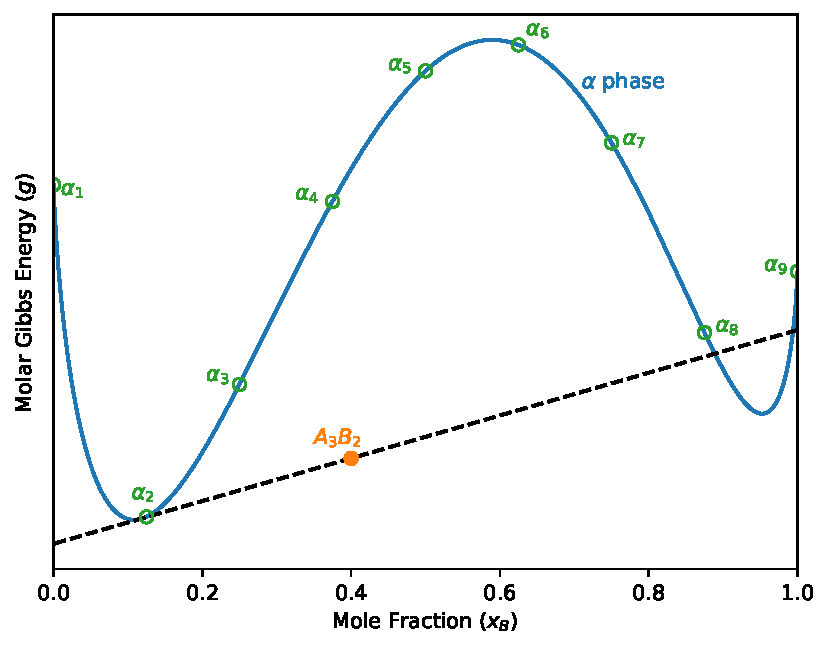
\includegraphics[width=0.65\textwidth]{figures/chapter-6/System_AB_grid.pdf}
		\caption{Demonstration of the grid construction method for fictive binary system in test problem A. The domain has been sampled at nine equispaced grid points and the pure stoichiometric phase \ce{A3B2} is found to be in equilibrium with the solution phase giving a false positive.}
		\label{fig:Grid_cons}
	\end{figure}

The discretisation of the grid plays a key role in the efficacy of this method and it has been shown by Chen \textit{et al.} \cite{Chen93b} that the grid must be sufficiently resolved to avoid missing critical features such as the minimum between grid points $\alpha_8$ and $\alpha_9$ in figure~\ref{fig:Grid_cons}. However, this requirement leads to performance concerns as too small a grid leads to an increase in the computational cost while too large a grid can lead to false positives in the optimisation process.  Piro and Simunovic \cite{Piro16} have demonstrated how uniformly spaced grid for a phase $\phi$ in $N_\phi$ dimensional Euclidean phase (each dimension corresponds to a species in phase $\phi$) can result in an enormously large number of grid points depending on the grid size. In the example with nine grid points, it becomes clear from figure~\ref{fig:Grid_cons} that global minimum would not be found but increasing the number of grid points will lead to an exponential increase in the cost. In conclusion, the rapid increase in the computational cost with the reduction in grid size and a questionable performance in terms of reaching a global maximum tilts the scales against this method. Despite the fact, this method was tested with three separate grid spacings ($\delta = 0.1, \, 0.01, \,\text{and}\, 0.001$) to serve as benchmarks and to numerically show the rapid increase in computational time.
	
	\subsection{Spatial branch \& bound (sBB)}
		The Branch and Bound (BB or B\&B), attributed to Land and Doig \cite{Land:1960aa} who introduced it in 1960 for discrete programming, is a widely used algorithmic paradigm for finding optimal solutions to optimisation problems. As illustrated in \ref{fig:BB},the algorithm systematically enumerates all the candidate solutions by sequentially pruning out non-feasible solution candidates through a recursive approach of partitioning the domain and finding an upper and a lower bound for each subdomain. In 1969, Falk and Soland \cite{Falk69} proposed one of the first BB algorithms that could be applied to an continuous objective function with separable concave portions with a closed and convex set of constraints and a bounded feasibility region.
		\begin{figure}[htbp]
		\centering
		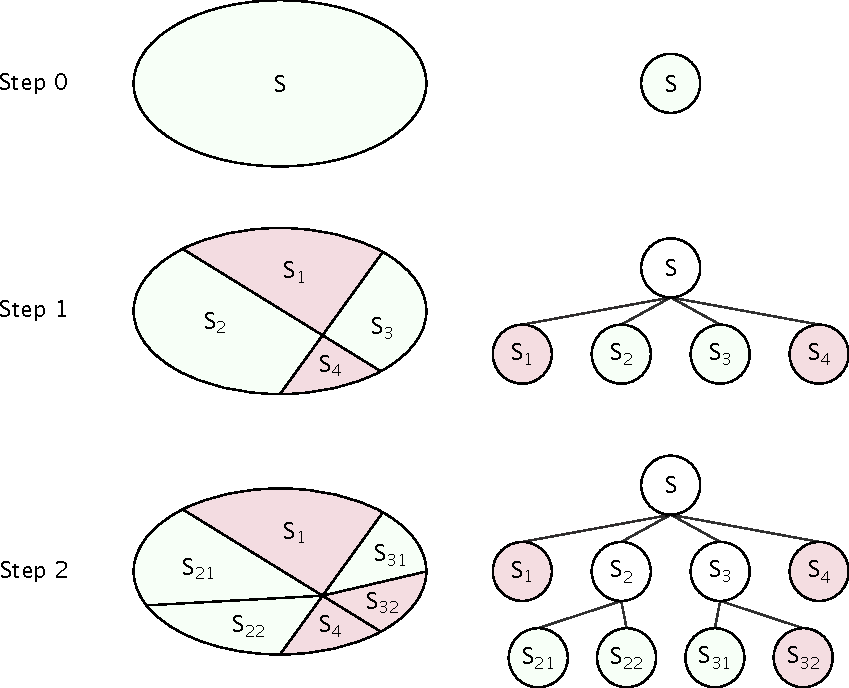
\includegraphics[width=0.65\textwidth]{figures/chapter-6/BB.pdf}
		\caption[Illustration of Branch and Bound (BB) class of algorithms.]{Illustration of the Branch and Bound (BB) class of algorithms. At each step, the domain is partitioned into a set of unexplored subdomains (denoted as nodes in a dynamic tree) which represent potential regions of optimal solution. By estimating the upper and lower bound on each subdomain, regions of infeasibility can be eliminated.}
		\label{fig:BB}
	\end{figure}
The BB algorithm involves two procedures to solve global optimisation problems:
	\begin{enumerate}
		\item \emph{Branching}: The domain $S$ is partitioned into two or more smaller disjoint domains $S_1,S_2,\dots,$ such that $S = S_1 \cup S_2 \cup \dots$ Thus, the partitioned objective function can be considered a convex approximation of the objective function within the subdomain $S_i$.
		\item \emph{Bounding}: The upper and lower bound of the objective function are found within a subset of the domain $S$. In the classical Branch and Bound method, a subdomain can be removed from the analysis if the lower bound of the objective function in it is greater than the upper bound of the objective function in any other subdomain.
	\end{enumerate}
McDonald and Floudas \cite{McDonald95} applied the BB algorithm to solve thermochemical equilibrium problems and Piro and Simunovic \cite{Piro16} proposed a modified version of the classical BB for the thermochemistry library {Thermochimica} which uses a different initialisation procedure and relaxation scheme for the bounds. Furthermore, instead of relying on pruning, every subdomain is evaluated till stopping criteria are met and if necessary, recursive partitioning technique is applied. The approach adopted by Piro and Simunovic \cite{Piro16} partitions the domain for each phase $\phi$ into $N_\phi$ subdomains and the driving force $\Delta G_\phi$ given by equation~\eqref{eq:DrivingForceLagrangian} is minimised in each subdomain. Their approach results in a Hessian which can be represented as a symmetric arrow matrix and by exploiting the structure of this matrix, the combination of $x_i$ that minimises $\Delta G_\phi$ can be easily determined. To solve the matrix, Gaussian elimination can be performed on the just the bottom row followed by back substitution. Furthermore, instead of storing a Hessian, the diagonal vector and a scalar representing the far right column can be stored. However, the implementation of this method warrants the use of an appropriate line search algorithm to ensure that the Wolfe conditions are satisfied and that the local system stays within the feasible region $0 < x_i <1$ . In addition, the step length must be suitably constrained to avoid missing any local minimums \cite{Piro16}. While the method works reasonably well, there are situations where it fails to correctly identify the true global minimum.

One of the best known method for solving non-convex nonlinear programming (NLP) problems is the \emph{spatial Branch and Bound (sBB)} \cite{Smith:1996aa,Tawarmalani:2013aa}. The branching, as already mentioned, is done by taking a continuous variable $v_i \in \left[v_i^l , v_i^u \right]$ and choosing $\beta \; (v_i^l \leq \beta \leq v_i^u)$ to create two subproblems with domains $\left[v_i^l , \beta \right]$ and $\left[\beta , v_i^u \right]$. When solving either subproblem, the original lower and upper bounds can be replaced by tighter bounds by taking the advantage of the reduced domain. This process, from McCormick \cite{McCormick:1976aa}, is called \emph{spatial branching}.
In this work, a \emph{Symbolic Reformulation sBB} \cite{Smith:1996aa,Smith:1997ab,Smith:1999aa} has been used through the Couenne (Convex Over and Under ENvelopes for Nonlinear Estimation) open-source software \cite{Belotti:2009aa,Belotti:2022aa}. Couenne has been developed to solve global optimisation problems $(\mathbf{P})$  of the form \cite{Belotti:2009aa}:
\begin{equation} \label{eq:couenne_prob}
\begin{aligned}
	\min \quad &f(x)			& \\
	\text{s.t.} \quad &g_j(x) \leq 0  	& &\forall j \in M \\
	&x_i^l \leq x_i \leq x_i^u	& &\forall i \in N_0 \\
	& x_i \in \mathbb{Z}		& &\forall i \in N_i^0 \subseteq N_0,
\end{aligned}
\end{equation}
where $f : \mathbb{R}^n \rightarrow \mathbb{R}$ and, $\forall j \in M$, $g_j : \mathbb{R}^n \rightarrow \mathbb{R}$ are multivariate functions, $n = \left|N_0\right|$ is the number of variables, and $x = (x_i)_{i \in N_0}$ is the n-vector variables. In the context of equilibrium thermodynamics, the problem in the form conformant to the above equation is as follows:
\begin{equation}
\begin{aligned}
	\min \; & \Delta G_\phi(x_i) = \sum_{i=0}^{N_\phi} \left( \tilde{\mu}_i - \sum_{j=1}^{C} \nu_{ij}\tilde{\Gamma}_j \right)		& \\
	\text{s.t.} \; &\sum_{i=1}^{N_\phi} x_i = 1  	& &\forall i \in N_\phi \\
			&\sum_{i=1}^{N_\phi} \nu_{i{e^-}} x_i = 0 & &\forall i \in N_\phi \\
	&0 \leq x_i \leq 1	& & \forall i \in N_\phi.
\end{aligned}
\end{equation}
Couenne implements linearisation, branching, heuristics and bound reduction and reformulates the problem by introducing a set of auxiliary variables. The reformulation of problem represented by equation~\eqref{eq:couenne_prob} results in the following form $(\mathbf{P'})$ \cite{Belotti:2009aa}: 
\begin{equation} \label{eq:couenne_reform}
\begin{aligned}
	\min \quad &x_{n+q}			& \\
	\text{s.t.} \quad &x_i = \vartheta_i \left(x \right)  	& &\forall i \in \{{n+1}, {n+2}, \dots, {n+q} \} \\
	&x_i^l \leq x_i \leq x_i^u	& &\forall i \in N \\
	& x_i \in \mathbb{Z}		& &\forall i \in N_i \subseteq N,
\end{aligned}
\end{equation}
where $N = \{{1}, {2}, \dots, {n+q} \}$ is the new variable index set which is a union of the original index set $\{{1}, {2}, \dots, {n} \}$ and the auxiliary index set $\{{n+1}, {n+2}, \dots, {n+q} \}$. $N_i$ denotes the index set of integer variables and the value of the last auxiliary variable, $x_{n+q}$, is the value of the objective function.

sBB algorithms rely on the generation of rigorous lower and upper bounds for the objective function value over any given variable subdomain. Generation of a upper bound is relatively simple as any feasible point of problem $(\mathbf{P})$ serves as an upper bound to the function at global minimum. In practice, it is best to chose the local minimiser of equation~\eqref{eq:couenne_prob} as the upper bound. When the reformulated problem $(\mathbf{P'})$ is in factorable form, the feature can be used to derive valid bounds and exact solution or one can use linear and quadratic approximations of $f$ and $g_j$. Detailed descriptions of sBB algorithms are found in literature \cite{Smith:1999aa,Liberti:2006aa} and the specifics to implementation in Couenne are described in \cite{Belotti:2009aa} but the method, illustrated in algorithm~\ref{alg:sBB}, is briefly described here. 
	
\SetKwComment{Comment}{/* }{ */}
\RestyleAlgo{ruled}
\begin{algorithm}[ht!]
	\caption[sBB algorithm for the MINLP problem $(\mathbf{P})$]{sBB algorithm for the MINLP problem $(\mathbf{P})$  \cite{Belotti:2009aa}}
	\label{alg:sBB}
	\KwIn{Problem $(\mathbf{P})$}
	\BlankLine
	Define set $L$ of subproblems, $L \gets \{\mathbf{P}\}$\;
	Define upper bound $z^u$ for $\mathbf{P}$,  $z^u \gets \infty$\;
	\While{$L \neq \emptyset$}{
		Choose $\mathbf{P}_k \in L$\;
		$L \gets L \setminus \{\mathbf{P}_l\}$\;
		Apply bound tightening to $\mathbf{P}_k$\ \Comment*[r]{Bound tightening}
		\If{$\mathbf{P}_k$ is feasible after bound tightening}{
  			Generate a linear relaxation $\mathbf{LP}_k$ of $\mathbf{P}_k$\ \Comment*[r]{Linearisation}
    			\Repeat{$\bar{x}^k$ is feasible for  $\mathbf{P}_k$ or  $\bar{z}^k$ does not improve}{
				Solve $\mathbf{LP}_k$ to get an optimum $\bar{x}^k$ with objective value $\bar{z}^k$\;
				Refine linearisation  $\mathbf{LP}_k$\;}
			\If{$\bar{x}^k$ is feasible for  $\mathbf{P}_k$}{$z^u \gets \min{\{z^u, \bar{z}^k\}}$\;}
    			Find a local optimum $\hat{z}^k$ of $\mathbf{P}_k$\ \Comment*[r]{Upper bound calculation}
			$z^u \gets \min{\{z^u, \hat{z}^k\}}$\;
			\If{$\bar{z}^k \leq z^u - \epsilon$}{
			Choose a variable $x_i$\ \Comment*[r]{Branching variable selection}
			Choose a branching point $x_i^b$\ \Comment*[r]{Branching point selection}
			Create subproblems:\\
				$\quad\mathbf{P}_{k-}$ with $x_i \leq x_i^b$,\\
				$\quad\mathbf{P}_{k+}$ with $x_i \geq x_i^b$\;
			$L \gets L \cup \{\mathbf{P}_{k-}, \mathbf{P}_{k+}\}$\;				
			}
  		}
  	}
	\BlankLine
	\KwOut{$z_\text{out} \gets z^u$, an optimal solution of $(\mathbf{P})$}
\end{algorithm}
	
\begin{enumerate}
	\item \emph{Reformulation}\\
		A general method for allowing the formation of convex relaxation for any continuous twice differentiable function was given in \cite{Androulakis:1995aa,Adjiman:1996aa,Adjiman:1997aa} and a tighter relaxation framework was developed by Smith and Pantelides \cite{Smith:1999aa}. The goal of reformulation is to construct an equivalent formulation $\mathbf(P')$ to problem $\mathbf(P)$ such that it contains only linear constraints and special non-linear definitions. Since convex relations of many transcendental functions (such as logarithms, exponentials, etc.) exist and most algebraic expressions, including the ones encountered in equilibrium thermodynamics, are made up of binary operations of arithmetic and the unary operators, it is possible to construct convex relaxations of any algebraic expression. For doing this, additional variables can be introduced in the problem. For example, in test problem A, the non-linear terms in the excess mixing part can be reformulated as a linear problem by introducing variables $w_1 = x_A x_B$ and $w_2 = x_A x_B^2$. Such a process can be generalised and automated using the standard binary tree representation of algebraic expressions \cite{Smith:1996aa}. The reformulated problem $\mathbf(P')$ is equivalent to the original problem $\mathbf(P)$ but all the non-linearities are described by sets corresponding to bilinear product, linear fractional, simple exponentiation and univariate function terms. Because the two problems are equivalent, a convex relaxation of $\mathbf(P')$ is also a valid relaxation of $\mathbf(P)$. Hence, reformulation allows constructing a convex relaxation of any problem and the sBB determined optimal solution of $\mathbf(P')$ is also the optimal solution to $\mathbf(P)$.
	
	\item \emph{Linearisation}\\
		If one considers the constraint $x_j = \vartheta_j(x)$ created during reformulation and set $B = [x^l, x^u]$ defining bounds on the variables, a $\vartheta_j$-linearisation is a system of linear inequalities $A^j x \geq b^j$ such that $X_\text{LP} := {x \in B : A^j x \geq b^j} \supseteq {x \in B : x_j = \vartheta_j(x)}$. If a $\vartheta_j$-linearisation is created for each constraint $x_j$, a linear problem $\mathbf{LP}_k := \min{x_{n+q} : Ax \geq b}$ is a linear relaxation of $\mathbf{P}_k$ where $\mathbf{P}_k$ is a root node of $\mathbf{P}$ obtained through branching. The optimal solution $\bar{x}$ of $\mathbf{LP}_k$ provides a lower bound for the problem. If the solution of $\mathbf{LP}_k$ becomes infeasible for $\mathbf{P}_k$, the lower bound can be improved by either branching or refinement of $\mathbf{LP}_k$, i.e. by amending linearisation inequalities \cite{Belotti:2009aa}. Couenne uses a variant of the projection error rule for refinement \cite{Belotti:2009aa}.
		
	\item \emph{Bound tightening}\\
	According to Smith and Pantelides \cite{Smith:1999aa}, sBB can  achieve convergence without any bound tightening but the rate of convergence can be improved by using it. The goal of bound tightening is to reduce the interval $[x_i^l, x_i^u]$ without causing the optimal value of the problem to change and it allows reduction of the feasible set and an improved linearisation. One way of propagating the effects of constraints to variable bounds in optimality-based bounds tightening (OBBT) \cite{Liberti:2006aa,Quesada:1995aa,Smith:1996aa} but faster-feasibility bounds tightening (FBBT) are also available albeit resulting in weaker bounds \cite{Liberti:2006aa,Smith:1996aa,Shectman:1998aa,Sahinidis:2003aa}. In OBBT, two convex optimisation problems are solved:
	\begin{align}
		x_i^l = \min_x x_i, \quad \text{subject to convex relaxation constraints}, \quad x^l \leq x \leq x^u, \\
		x_i^u = \max_x x_i, \quad \text{subject to convex relaxation constraints}, \quad x^l \leq x \leq x^u.
	\end{align}
OBBT can be applied to every variable $x_i$ separately and when feasible the convex relaxation constraints can be updated but at each iteration it will solve $2N$ optimisation problems making it extremely expensive and suitable only for initial bound tightening steps \cite{Smith:1999aa}. FBBT, on the other hand, considers each constraint of the  reformulated problem individually \cite{Shectman:1998aa}. At any sBB node $k$, if the local minimum $\hat{x}^k \in \left[x^l, x^u\right]$ of the convex relaxed problem $\mathbf{CP}_k$ is known, FBBT is applied to fictitious bounding box $B \cap {x \in \mathbb{R}^{n+q} : x_i \leq \tilde{x}_i}$, where $\tilde{x}_i \in \left(x_i^l, \hat{x}_i^k\right)$ is suitably chosen. If the resulting problem become infeasible or if its lower bound becomes larger than the best upper bound, then $\left[\tilde{x}_i^k, x_i^u\right]$ is a valid tightening . On the other hand, if $\tilde{x}_i \in \left(\hat{x}_i^k, x_i^u\right)$ is chosen and FBBT applied to the analogous bounding box results in infeasibility, then $\left[x_i^l, \tilde{x}_i^k\right]$ is valid.
	
	\item \emph{Branching}\\
		Branching is critical to the performance of sBB and an effective strategy can help minimise the size of the sBB tree. The goal of branching is to choose a branch variable and corresponding branch point to be use to partition the domain. In doing so, the goal must be to improve the lower bound of the resulting subproblems and to eliminate as large an infeasible region as possible. In doing so, one must also try to keep the sBB balanced and together the three requirements are often conflicting and the implementations can be optimised to emphasise on one aspect or the other. Branching may be required when the lower bound $\bar{x}_{n+q}^k$ of an sBB node $\mathbf{P}_k$ is smaller than the best known feasible solution and the relaxation $\mathbf{LP}_k$ cannot be further refined. To objectively select the branching variable and point, Belotti \textit{et al.} \cite{Belotti:2009aa} define the $\vartheta_i$-\textit{infeasibility} of auxiliary variable $x_i$ at node $k$ as $U_i\left(\bar{x}^k\right) = \left|\bar{x}_i^k - \vartheta_i\left(\bar{x}^k\right) \right| \slash \left(1 + \left \Vert \nabla \vartheta_i(\bar{x}^k)  \right \Vert_2\right)$. The scaling of the error term in numerator with the norm of the gradient avoids selecting a variable $x_i$ with a small bound interval $[x_i^l, x_i^u]$ but with a large $\left|\bar{x}_i^k - \vartheta_i\left(\bar{x}^k\right) \right|$ as it is unlikely to improve linearisation if used for branching.
		\begin{enumerate}
			\item	Branching variable selection\\
				In Couenne, integer variables have higher priority than continuous variable but since the driving force function results in a strictly NLP problem, continuous variables become the only candidate for branching. Defining the \emph{dependence set}, $D(x_i)$, as the set of variables in $\vartheta_i(x)$ (these are the variables in $x$ that $x_i$ directly depends on), the infeasibility of variable $x_i$ can be propagated to $D(x_i)$. In Couenne, Belotti \textit{et al.} \cite{Belotti:2009aa} define the non-linear infeasibility as:
				\[
					\Omega_i^N(\bar{x}^k) = \mu_1 \sum_{j\in E(i)} U_j(\bar{x}^k) +  \mu_2 \max_{j\in E(i)} U_j(\bar{x}^k) +  \mu_3 \min_{j\in E(i)} U_j(\bar{x}^k),
				\]
				where for variable ${x}_i$, the set $E(i) = {j \in N \; : \; x_i \in D(x_j)}$. Parameter $\mu_k \geq 0, \, k = 1, 2, 3 $\footnote{Parameters $\mu_k$ defined here have no correlation to the chemical potential $\mu_i$.} and $\mu_1 + \mu_2 > 0$ ensures that $\bar{x}^k$ is infeasible if and only if $\Omega_i^N(\bar{x}^k) > 0$ for at least one variable $x_i$. In Couenne $(\mu_1, \mu_2, \mu_3) = (0.1, 1.3, 0.8)$ \cite{Belotti:2009aa}. The strategy, however, can often be ineffective and Couenne also has implementations of \emph{Violation Transfer} proposed by Tawarmalani and Sahinidis \cite{Tawarmalani:2004aa} and an extension of the \emph{reliability branching} technique introduced by Achterberg \textit{et al.} \cite{Achterberg:2005aa}. In violation transfer, violations of non-convexities by the current solution are assigned to problem variables followed by transfer of violations to $D(x_i)$.  The. violations are then weighted to account for branching priorities and potential for convex relaxation improvement. The variable that leads to the maximum weighted violation is selected as the branching variable \cite{Tawarmalani:2004aa}. Since, the reliability branching strategy was not used in {\GEM}, a discussion of it is omitted and can be found in \cite{Belotti:2022aa}.
			\item Branching point selection\\
				For a continuous variable $x_i$ appearing in a single expression $x_j = \vartheta_j(x_i)$, the goal of sBB is to keep the resulting tree balanced. This makes areas of the linearisations a reasonable metric for selecting the branching point as shown in figure~\ref{fig:branching_pt}. In Couenne, three branching point selection strategies are implemented.
				\begin{figure}[htbp]
					\centering
					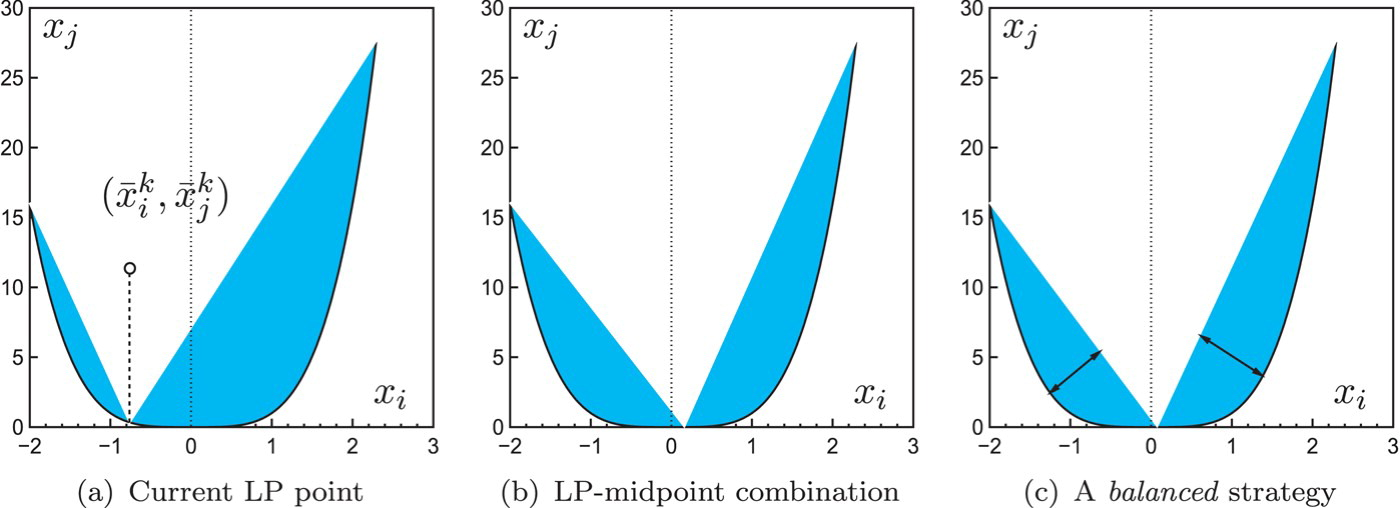
\includegraphics[width=\textwidth]{figures/chapter-6/branching_point}
					\caption[Strategies for selecting a branching point]{Strategies for selecting a branching point as implemented in Couenne: (a) branching on current LP solution $\bar{x}_i^k$, (b) Convex combination of LP point $\bar{x}_i^k$ and midpoint of bound interval, (c) Balancing the areas of the two resulting linearisations. Figure from Belotti \textit{et al.} \cite{Belotti:2009aa}.}
			\label{fig:branching_pt}
			\end{figure}
		
		In the \emph{LP-based strategy}, the branching point is set so that $\bar{x}^k$ can become infeasible in both the subproblems. While simple to implement, as shown in subfigure (a) of figure~\ref{fig:branching_pt}, it can result in unbalanced subproblems. To avoid this, for variable $x_i \in [x_i^l, x_i^u]$, the branching point can be set as a convex combination of $\bar{x}_i^k$ and the midpoint of bound interval, $x_i^m = (x_i^l + x_i^u) / 2$ (see subfigure (b) of figure~\ref{fig:branching_pt}). Hence, a selection strategy guaranteeing a minimum distance from variable bounds is as follows \cite{Tawarmalani:2013aa}:
		\[
			x_i^b = \max \left \{x_i^l +b, \min \left \{x_i^u -b, \alpha \bar{x}_i^k + \left(1-\alpha\right)x_i^m \right \} \right \},
		\]
		where $0 < \alpha < 1$ and $b = \beta(x_i^u - x_i^l)$ for $0 < \beta < 0.5$ and $\alpha$ and $\beta$ are set to \num{0.25} and \num{0.2} respectively \cite{Belotti:2009aa} and  the strategy tries to balance the half-intervals of $x_i$. Alternatively, if a local minimum $\hat{x}^k$ is known, $\hat{x}_i^k$ can be chosen as a branching point since the resulting convexification will return a solution $\bar{x}^k$ that is very close to $\hat{x}^k$ \cite{Shectman:1998aa}.
		
	In \emph{expression-based strategies}, one can aim to reduce the sum of the areas of the resulting convexifications as shown in subfigure (c) of figure~\ref{fig:branching_pt}. Several methods for such strategy can be adopted \cite{Kalantari:1987aa,Liu:1996aa} but a balanced strategy implemented in Couenne finds the branching point using a binary search on the interval $[x_i^l, x_i^u]$ that minimises the difference between the maximum area $u'(x_i)$ and maximum area $u''(x_i)$ \cite{Belotti:2009aa}:
	\[
		x_i^b \in \argmin \left | \max_{x_i \in [x_i^l, x_i^b]} u'(x_i) - \max_{x_i \in [x_i^b, x_i^u]} u''(x_i) \right|,
	\]
	where $u'$ and $u''$ are the distance between the upper envelope line of $\vartheta_j$ and $(x_i, \vartheta_j(x_i))$ on the subdomains LP' and LP'' resulting from branching. The method balances the maximum distance between the points on $\vartheta_j(\cdot)$ and the upper envelope \cite{Belotti:2022aa}.
		\end{enumerate}	
\end{enumerate}

	  Together, the reformulation of the problem and the sBB algorithm result in a rigorous solution framework for global optimisation problem. Since the driving force functions are smooth and differentiable, they are well formulated for the method. Though the reformulation results in an increase in the size of the problem, it doesn't become a major issue for determining the minimum of the driving force.
	  
	
	\subsection{Particle swarm optimisation}
	
	Particle swarm optimisation (PSO) is a stochastic search algorithm inspired by the flocking behaviour of birds. First proposed by Kennedy and Eberhart \cite{Eberhart:1995aa,Kennedy95}, PSO is a population based method which relies on the premise of social sharing of information among a bird flock seeking food. PSO is relatively simple to describe and implement and its apparent competence in finding optimal solutions in complex search spaces has made it a widely studied search algorithm \cite{Freitas:2020aa}. In PSO, a population of candidate solutions, dubbed particles, moves around the search space as a function of the position and velocity of the particle and the movement of each particle is influenced by its best known local position and guided towards the best global position as other particles find better solutions. 

	At each iteration $t$, the velocity vector of particle $i$ in the swarm gets updated according to the following equation \cite{Bonyadi:2017aa}:
	\begin{equation} \label{eq:PSO_vel}
		\mathbf{v}_i^{t+1} = \omega \mathbf{v}_i^{t} + \psi_i {R_1}_i^t \left( \mathbf{p}_i^{t} - \mathbf{x}_i^{t} \right) +\psi_i {R_2}_i^t \left( \mathbf{g}^{t} - \mathbf{x}_i^{t} \right),
	\end{equation}
	where $\mathbf{v}_i^t$ and $\mathbf{x}_i^t$ are the velocity and position at iteration $t$. The inertia weight is given by $\omega$ and $\psi_1$ and $\psi_2$ are real acceleration coefficients known as cognitive weight and inertia weight respectively. Together, the weights control the impact of global and individual best positions on the particle's velocity and trajectory. Kennedy and Eberhart \cite{Kennedy95} originally assigned the same value of \num{2} to social and cognition parts but fine-tuning the parameters is critical to performance and convergence of PSO, particularly when dealing with multimodal problems \cite{Carlisle:2001aa,Trelea:2003aa,van-den-Bergh:2006aa}. $R_1$ and $R_2$ are uniformly distributed vectors used to maintain an adequate level of diversity in the swarm population and $\mathbf{p}_i^{t}$ and $\mathbf{g}^{t}$ represent the best known position of particle $i$ and the global best position of the swarm at iteration $t$. In turn, the position of each particle $i$ at every iteration $t$ can be updated according to the following equation \cite{Bonyadi:2017aa}:
	\begin{equation}  \label{eq:PSO_pos}
		\mathbf{x}_i^{t+1} = \mathbf{x}_i^{t} + \mathbf{v}_i^{t}.
	\end{equation}
	
	\SetKwComment{Comment}{/* }{ */}
\RestyleAlgo{ruled}
\begin{algorithm}[ht!]
	\caption[PSO algorithm for objective function $f : \mathbb{R}^n \rightarrow \mathbb{R}$]{PSO algorithm for objective function $f : \mathbb{R}^n \rightarrow \mathbb{R}$}
	\label{alg:PSO}
	\KwIn{Objective function $f$, Search space $\mathbf{x}_i = \left[\mathbf{x}_i^l, \mathbf{x}_i^u\right]$, Number of particles $N_p$}
	\BlankLine
	\For{Particle $i \in \{1, 2, \dots, N_p\}$}{
		Initialise initialise position, $\mathbf{x}_i \gets \mathcal{U}\left(\mathbf{x}_i^l, \mathbf{x}_i^u\right)$\;
		Initialise particle's best known position, $\mathbf{p}_i \gets \mathbf{x}_i$\;
		\If{$f(\mathbf{p}_i) < f(\mathbf{g})$}{
			Update global best position, $\mathbf{g}_i \gets \mathbf{p}_i$\;
		}
		Initialise the particle velocity, $\mathbf{v}_i \gets \mathcal{U}\left( - \left | \mathbf{x}_i^u - \mathbf{x}_i^l \right |, \left | \mathbf{x}_i^u - \mathbf{x}_i^l \right | \right)$\; 
	}
	\While{Termination criteria is not met}{
		\For{Particle $i \in \{1, 2, \dots, N_p\}$}{
			Pick random vectors, $\mathbf{R}_1, \mathbf{R}_2 \gets \mathcal{U}\left(0, 1\right)^n$\;
			Update particle velocity, $\mathbf{v}_i^{t+1} \gets \omega \mathbf{v}_i^{t} + \psi_i {R_1}_i^t \left( \mathbf{p}_i^{t} - \mathbf{x}_i^{t} \right) +\psi_i {R_2}_i^t \left( \mathbf{g}^{t} - \mathbf{x}_i^{t} \right)$\;
			Update particle position, $\mathbf{x}_i^{t+1} = \mathbf{x}_i^{t} + \mathbf{v}_i^{t}$\;
			\If{$f(\mathbf{x}_i^{t+1}) < f(\mathbf{p}_i) $}{
				Update particle's best known position, $\mathbf{p}_i^t \gets \mathbf{x}_i^{t+1}$\;
				\If{$f(\mathbf{p}_i^t) < f(\mathbf{g})$}{
				Update global best position, $\mathbf{g}^t \gets \mathbf{p}_i^t$\;
			}	
		}
	}
	}
	\BlankLine
	\KwOut{$x_\text{out} \gets \mathbf{g}^t$, an optimal solution of $f$}
\end{algorithm}

	The PSO algorithm, illustrated algorithm~\ref{alg:PSO}, has several advantages compared to other continuous optimisation methods. First, PSO is a problem independent algorithm which only needs the objective function to evaluate the fitness of each candidate solution. In doing so, PSO does not make any assumptions about the continuity and differentiability of the objective function. Second, the evolution of particles is random and therefore the gradients of the objective function need not be calculated. Lastly, PSO does not need a good initial estimate or a-priori knowledge of the objective function search space \cite{Freitas:2020aa}. These factors have led PSO to gain a widespread appeal and it has shown good performance in several domains like function optimisation, artificial neural network training, fuzzy system control, etc. Unfortunately, for complex multimodal problems, the conventional PSO algorithm can get trapped in local optima, considerably compromising the convergence rate. This leads to poor performance and accuracy, and imposes restrictions on applicability to a wide range of practical problems \cite{Xu:2013aa,Harrison:2018aa}. While a-priori tuning can help improve performance, it is a time-intensive process but also assume that the optimal parameter configuration does not change over time. However, as shown by Leonard and Engelbrecht \cite{Leonard:2013aa}, the parameter values well-suited for exploration are not well-suited for exploitation and vice-versa. To achieve the two fold characteristic of good convergence speed and to avoid stagnating in local optima, several variations of PSO have been developed \cite{Shi:1998aa,Ratnaweera:2004aa,Chatterjee:2006aa,Fan:2007aa,van-den-Bergh:2001aa}. Another limitation of PSO is in constrained optimisation problem as it lacks an explicit constraint-handling mechanism. Several methods such as penalty function, feasibility-based rules method and the constraint-preserving method have been proposed with the penalty method being the most commonly used \cite{Sun:2011aa,Jordehi:2015aa}. While detailed discussions on handling these problems are available in open literature, the specific approach in the context of this work is discussed in the following text. 	
	
	\begin{enumerate}
		\item \emph{Constraint handling}\\
			As previously stated, several strategies have been explored to impose the constraints in PSO. One of the simplest constraint-handling mechanism is that of reseting the particles that escape the feasible region \cite{Hu:2002aa,Guo:2004aa,Sun:2009aa}. Minimisation of a non-stationary multi-stage assignment penalty function was proposed by Parsopoulos and Vrahatis \cite{Parsopoulos:2005aa} and the results were promising albeit at the cost of a very complex process for determining penalty. In the feasibility-based approaches such as that by Pulido and Coello \cite{Pulido:2004aa}, a candidate solution is chosen leader based on Deb's comparison rules \cite{Deb:2000aa}. The constraint handling strategy implemented in {\GEM} is based on the method by Hu and Eberhart \textit{et al.} \cite{Hu:2002aa}. To make the solution more plausible, all the equality constraints are modified into inequality constraints to specified tolerance, i.e., the constraints on sum of mole fractions and the charge neutrality constraints are reformulated as:
			\begin{gather}
				\left | \sum_{i=1}^{N_\phi} x_i - 1 \right | <  \epsilon_1,\\
				\left | \sum_{i=1}^{N_\phi} \nu_{i{e^-}} x_i \right | < \epsilon_2.
			\end{gather} 
			The initialisation step is then modified to impose the constraints and once a feasible initial solution is found, the algorithm can progress. At every iteration $t$, each particle is checked for feasibility. If the updated position $x_i^{t+1}$ results in the bounds being violated, the step length is updated based on the following equation:
			\begin{equation}  \label{eq:PSO_pos_alpha}
				\mathbf{x}_i^{t+1} = \mathbf{x}_i^{t} + \alpha \mathbf{v}_i^{t},
			\end{equation}
			where $\alpha \in \mathcal{U} (0.1, 0.9)$ is a randomly generated constriction vector used to scale the step length. Handling the constraints, however is less straightforward. Once the position of each particle has been updated, the feasibility of each particle is verified and if it is found to violate the feasibility condition, Deb's comparison rules \cite{Deb:2000aa} are applied as follows:
			\begin{enumerate}
				\item	If all candidate solutions are infeasible, the candidate closest to feasibility is selected as the best candidate and the remaining particles are restored to previous feasible position. The best known position of these particles is not changed.
				\item If some candidates are feasible, their personal best is updated and the global best solution is selected from the feasible particles. The particles in infeasible regions are restored to the previous feasible solution.
				\item If all candidates are feasible, the same process as usual is followed.
			\end{enumerate}
			
		\item \emph{Particle initialisation}\\
			One of the parameters in PSO that can potentially affect the convergence rate is the number of particles and their initial positions. While the particle position $x_i$ is often initialised randomly from a uniform sampling in $\left[ x_i^l, x_i^u\right]$, it has been shown by Woronow \cite{Woronow:1993aa} that, when compared to normalised exponential distribution, normalised uniform distributions produce a poorer coverage of composition space. Otis \textit{et al.} \cite{Otis:2017ab} employed a set of different sampling strategies such as Halton sequence, Sobol sequence and their variations to come come up with an efficient sampling strategy for PyCalphad. Furthermore, Piro and Simunovic \cite{Piro16} found that PSO often fails to capture the optimal solutions located close to the domain edges and special considerations must be taken when the optimal solution may exist close to the boundaries. To best see the effect of particles' initial position on the performance of PSO, a number of different options were tested. First, the number of particles, $N_p$, was selected from a finite set $\left\{ N_\phi, 2N_\phi\right\}$ and second, the particles were initialised using both normalised uniform and normalised exponential sampling. In addition, when $N_p = 2N_\phi$, a hybrid strategy was also used where $N_\phi$ particles were initialised using the sampling methods while the remaining $N_\phi$ particles were fixed at the corners of the domain. The reasoning behind this approach is that the particles closer to the edges should enable the spare closer to the edges to be properly explored. Also, more advanced sampling methods were not selected as, with well-tuned hyperparameters, PSO is expected to efficiently scan the domain unlike when only sampling is used and one must make sure that the features are not missed if the samples are not well picked. 

		\item \emph{Particle dynamics}\\
			Parameter tuning can have a significant impact on the performance of PSO and a large number of \emph{Adaptive PSO} (APSO) algorithms have been proposed in literature to overcome the problem of a-priori tuning of the parameters. A comparative analysis of many such algorithms has been performed by Harrison \textit{et al.} \cite{Harrison:2018aa}. Amongst one of the promising APSO algorithms is \emph{APSO based on velocity information} (APSO-VI) proposed by Xu \cite{Xu:2013aa} which adapts the inertia weight based on the current velocity of the particles. The concept of APSO-VI is borrowed from Yasuda \textit{et al.} \cite{Yasuda:2008aa} and aims to evolve the velocity to be close to an \emph{ideal} velocity. In APSO-VI the average velocity of swarm is defined as \cite{Xu:2013aa}:
			\begin{equation}
				\bar{v}^t = \frac{1}{n N_p} \sum_{i=1}^{N_p} \sum_{i=1}^{n} \left | v_{ij}^t \right |,
			\end{equation}
			where $n$ and $N_p$ represent the problem dimension and the number of particles in the swarm respectively. The size of the average velocity reflects the size of the particle search space and to better explore the search space, one should maintain a larger average velocity with longer time, during the early stage of the optimisation. On the other hand, during the latter stage, it is important to keep a small average velocity to find the optimum solution efficiently \cite{Xu:2013aa}. One can then define an ideal velocity at iteration $t$, which decreases with time, as follows:
			\begin{equation}
				{v}_\text{ideal}^t = v_s \left(\frac{1 + \cos\left (\frac{\pi t}{T_\text{end}} \right )}{2} \right),
			\end{equation}
			where $v_s = (x^u - x^l) / 2$ is the initial ideal velocity, $T$ is the maximum number of iterations and $T_\text{end} = 0.95 T$ is the time in which 95\% of search is completed. As visualised in figure~\ref{fig:APSO-ideal_v}, the ideal velocity profile matches the requirements for an effective exploration of the search space.
			\begin{figure}[htbp]
				\centering
				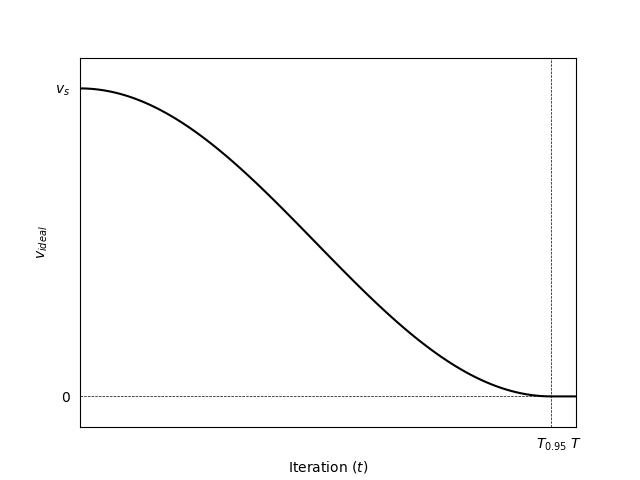
\includegraphics[width=0.75\textwidth]{figures/chapter-6/APSO-VI}
				\caption{Schematic of ideal velocity profile in APSO-VI.}
				\label{fig:APSO-ideal_v}
			\end{figure}
			The inertia weight can then be dynamically adapted at each iteration based on the average velocity in relation to the ideal velocity \cite{Harrison:2018aa} using:
			\begin{equation}
				\omega^{t+1} =  \begin{cases}
								\max \left\{ \omega^t - \Delta \omega, \, \omega_\text{min}\right\}& \text{if } \bar{v}^t \geq  {v}_\text{ideal}^{t+1}\\
								\min \left\{ \omega^t - \Delta \omega, \, \omega_\text{max}\right\}& \text{if } \bar{v}^t <  {v}_\text{ideal}^{t+1}
							\end{cases},
			\end{equation}
			where $\omega_\text{min}$ and $\omega_\text{max}$ are the minimum and maximum inertia weights and $\Delta \omega$ is the inertia weight step size. It has been shown by Harrison \textit{et al.} \cite{Harrison:2016aa} that decreasing the ideal velocity decrease the inertia weight such that it remains within convergent range. Xu fixed the parameters $\omega_\text{min} = 0.3$, $\omega_\text{max} = 0.9$, $\Delta \omega = 0.1$, and $\psi_1 = \psi_2 = 1.49$ \cite{Xu:2013aa} and, in this work, APSO-VI has been adopted, albeit with slightly different parameter values. In {\GEM}, the APSO-VI hyperparameters were selected to be $\omega_\text{min} = 0.2$, $\omega_\text{max} = 0.9$, $\Delta \omega = 0.1$, $\psi_1 = 1.5$ and  $\psi_2 = 2$. These values provided good convergence rates while reasonably exploring the search space and are similar to those previously used in thermodynamic equilibrium application such as by Piro and Simunovic \cite{Piro16} and Myint \textit{et al.} \cite{Myint:2021aa}.
	\end{enumerate}

	
	\subsection{Implementation and analysis}
	All global optimisation methods have their advantages and disadvantages and no global optimisation method is universally superior to others. While the deterministic methods are good at converging to a local minimum, they are often prone to high computational expenses. The stochastic methods, on the other hand, tend to cover the search space more effectively but face difficulty at finding the global minimum \cite{Piro16}. The global optimisation methods discussed in literature have mostly been problem centric and there has been a lack of a comprehensive and rigorous analysis of these methods applied to a variety of thermodynamic equilibrium problems. 	Since the global optimisation methods are critical to the performance of {\GEM}, an experimental approach was adopted to select method to be used. While the goal of the global minimiser can be restricted to identifying whether or not a phase has a negative driving force, in terms of comparison, the aim was to correctly identify the minimum of driving force in each of the eight test cases described in section~\ref{sec:test_global}.  
	
	Since, the convergence criteria for Couenne and the APSO-VI implementation differ, they must be clarified. In Couenne, the convergence is based on the feasibility tolerance. If a constraint $g_i(x) \leq 0$ within this tolerance, it is deemed satisfied \cite{Belotti:2022aa}. The Couenne solve requires several options to be specified. The ones of particular concern here were that related to branching for which violation transfer was selected and FBBT was applied to bound tightening. Since OBBT is computationally expensive, it was disabled and Couenne was allowed to use heuristics through interior point optimisation. The tolerance was left to the default value of ${10^{-6}}$.
	
	In APSO-VI, the convergence criterion is more complicated due to the stochastic nature of the algorithm. Guaranteeing that all the particles will converge to the same value is impossible without significantly compromising performance. Apart from a preset maximum number of iterations $T = 100$, the algorithm is deemed to converge if 95\% of the particles converge to a small distance of the global best position. For this, the Euclidean distance of each particle from the best known global solution is calculated using $S_i^t = \left \Vert x_i^t - g^t\right \Vert$ and if $S_i^t \leq 10-6$ for $0.95 N_p$ particles, the algorithm is terminated as converged. For calculating the Euclidean distance, only feasible solutions are considered and if a feasible global best is not identified, the algorithm is marked as failed.
	
	For comparison, each implementation of the method was executed a hundred times on a 2020 M1 MacBook Air with 8 GB of memory. The methods were alternated in ABC...ABC... pattern to avoid bias and the total time for all the runs was considered. The average time of all the times in the interquartile range was selected as the performance metric while the number of times the algorithm correctly identified the minimum or absence of negative driving force was the metric of reliability. No runs were discarded for the reliability metric. The results of a comparative analysis are shown in figures~\ref{fig:res_time} and \ref{fig:res_rel}. The results demonstrate that the equispaced grid sampling method is only effective with very small resolutions leading to a very rapid increase in the cost. On the other hand, the APSO is a lot more robust but they do show that a larger number of particles can better scan the space. Despite their efficiency, the robustness of the APSO is slightly lower than the sBB algorithm which converges to the correct results for each test case but does so at the cost of increase in computational time. 

\begin{figure}
     \centering
     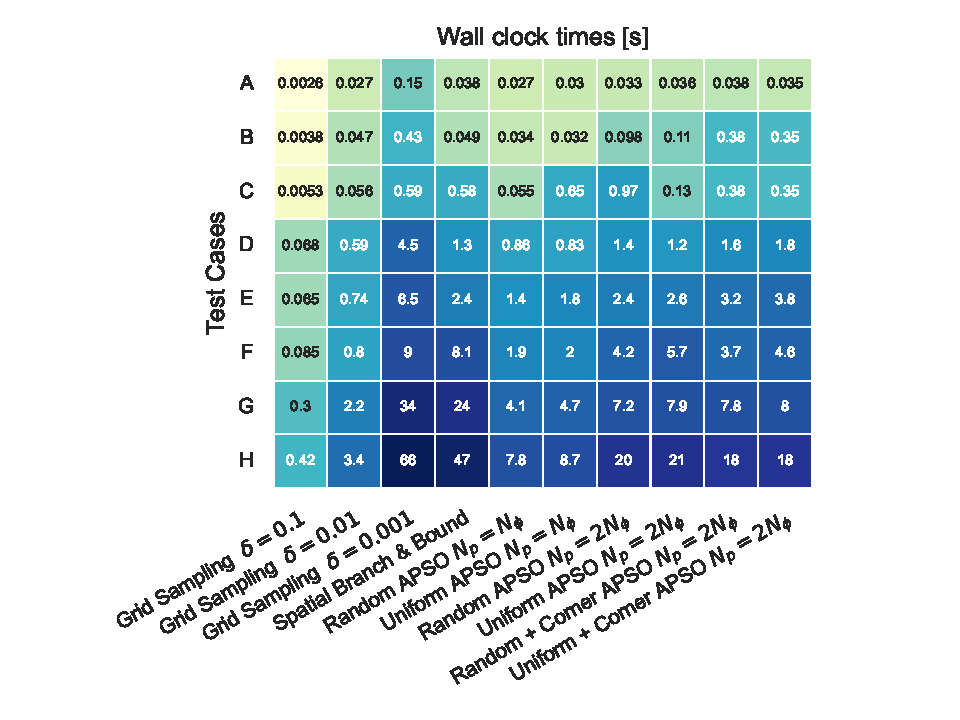
\includegraphics[width=0.6\textwidth]{figures/chapter-6/time.pdf}
     \caption[Comparison of computational performance of different global optimisation algorithms.]{Comparison of computational performance of various global optimisation algorithms for the test cases. The wall clock time is the average time of the results in interquartile range for 100 calculations of each method and case combination}
     \label{fig:res_time}
 \end{figure}



\begin{figure}
         \centering
         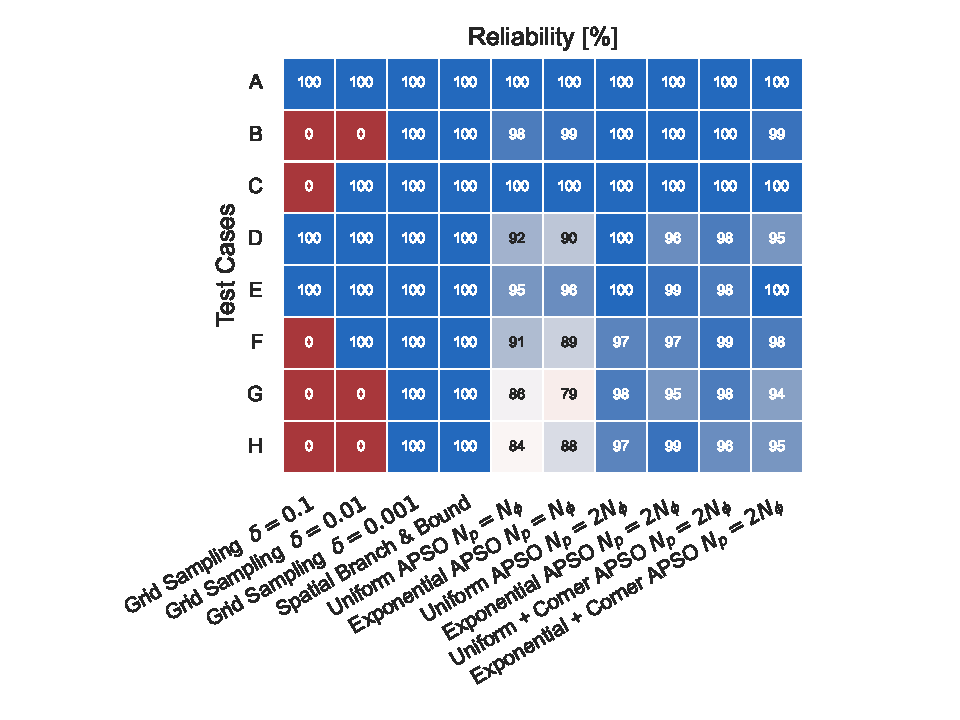
\includegraphics[width=0.6\textwidth]{figures/chapter-6/reliability.pdf}
         \label{fig:res_rel}
     	\caption[Comparison of reliability of different global optimisation algorithms.]{Comparison of reliability of various global optimisation algorithms for the test cases. The reliability is the number of times the correct results were shown by a method out of the 100 calculations.}
 \end{figure}
 
The grid sampling method was able to find the minimum in all the test cases albeit only when the grid resolution was increased to $\delta = 0.00$ and with a significant impediment on performance. In particular, one must be careful about the charge neutrality constraints with this approach. When dealing with ionic phases, many of the samples using this strategy will result in infeasibility due to the charge neutrality constraint getting violated. This can potentially compromise the method's reliability as a feasible point satisfying the charge constraint might never be found. In the implementation here, the objective function was evaluated at every sample point despite some of them being infeasible.

Among the tested options, sBB proves to be the most reliable though at a cost to performance. This is expected for the well behaved driving force functions. One way of reducing the computational cost of sBB is to terminate the solver as soon as an upper bound becomes negative or a feasible solution with negative driving force has been identified. This however has not been implemented in {\GEM}. The stochastic methods on the other hand exhibit fairly good computational performance though with a slightly lower reliability. In the experiments, the loss of reliability is attributable to reaching maximum iterations and in a small number of cases to converging to an infeasible value. Moreover, the impact of the number of particles in the swarm is clearly visible. With $N_p = N_\phi$, the space is not sufficiently scanned leading to a lower overall reliability. In such a scenario, increasing the number of particles seems to be the best choice but one must take cognisance of the fact that this can increase the computational time and might also require adjusting the convergence criteria. Initialising the particles on the corners did not have as big an impact as the number of particles. This can be attributed to the test cases itself where the optimal solution in most cases was not close to any edge and therefore no significant benefit was obtained from the particles scanning the space closer to the boundaries.

In the context of {\YJ}, both the sBB and APSO algorithms have been integrated into the code and the user will have the option of specifying the desired method. In cases where reliability is of the utmost and the system is deemed too complex, one could select sBB as the global optimisation algorithm while in cases where the system is deemed to be not very complicated or where there is a possibility of a-posteriori checking the results and / or augmenting global optimisation results with other information such as that from the grain information available in phase field.
	

\section{Summary}
	A number of algorithms for different parts of a thermodynamic equilibrium solver were presented in this chapter. Many of these algorithms have already been implemented in other codes available in the literature and GEM and levelling are relatively mature algorithms with little to no scope of improvement. This is evident from the fact that most of the development efforts since the original GEm method has relied on auxiliary operations such as initialisation, etc. However, this does not mean that improvements can not be made.  The development of an advanced thermodynamic solver leaves the door open for incremental gains on many of these algorithms.
For example, the post-levelling and temporal series estimates for initialisation will be more carefully analysed and implemented during this work in order to minimise the computational cost of the non-linear step. The work on non-linear step will focus on improving the convergence rate by focussing the attention on the line-search and phase update algorithms. Finally, two of the major areas that stand to benefit from this work are global optimisation methods and integration with multiphysics framework {MOOSE}. The rigorous application based study of global optimisation methods which will be performed during this work is expected to provide a definitive answer to the question of reliability, efficiency and robustness of various candidate methods for application to thermodynamic equilibrium problems. The optimum method will then be implemented to achieve the best possible performance. Regarding {MOOSE} integration, this work will try to minimise the costs associated with thermodynamic equilibrium calculations, which significantly impede performance of multiphysics simulations, by minimising thermodynamic computation costs themselves  and reducing overheads  related to coupling which also contribute towards the performance impediment.
